% ============================================================
%  DS200.Q21 — Tái triển khai và Cải tiến ViHateT5
%  cho Phát hiện Ngôn từ Thù ghét Tiếng Việt
%  Beamer Presentation — Nhóm 02 (Tiếng Việt)
% ============================================================
\documentclass[11pt, aspectratio=169]{beamer}
\usetheme{Frankfurt}
\usefonttheme{serif}

% --- Vietnamese ---
\usepackage{fontspec}
\setmainfont{texgyretermes}[
    Extension      = .otf,
    UprightFont    = *-regular,
    BoldFont       = *-bold,
    ItalicFont     = *-italic,
    BoldItalicFont = *-bolditalic
]
\usepackage{polyglossia}
\setdefaultlanguage{vietnamese}

% --- Packages ---
\usepackage{tikz}
\usetikzlibrary{arrows.meta, positioning, shapes.geometric, fit, calc}
\usepackage{amsmath,amssymb,graphicx,booktabs}
\usepackage{hyperref}
\usepackage[table]{xcolor}
\hypersetup{colorlinks=true,urlcolor=blue}
\usepackage{listings}
\usepackage{multicol}
\usepackage{caption}
\usepackage{multirow}
\usepackage{array}
\usepackage{colortbl}

\setbeamerfont{caption}{size=\tiny}
\setbeamertemplate{caption}[numbered]

% --- Main colors ---
\definecolor{uitblue}{RGB}{0,70,140}
\definecolor{uitdarkblue}{RGB}{0,50,100}
\definecolor{uitlightblue}{RGB}{220,235,250}
\definecolor{successgreen}{RGB}{40,140,40}
\definecolor{alertorange}{RGB}{210,105,30}

\setbeamercolor{structure}{fg=uitblue}
\setbeamercolor{frametitle}{fg=white,bg=uitblue}
\setbeamercolor{title}{fg=white, bg=uitblue}
\setbeamercolor{block title}{bg=uitblue!80,fg=white}
\setbeamercolor{block body}{bg=blue!5,fg=black}
\setbeamercolor{section in head/foot}{fg=white, bg=uitblue}
\setbeamercolor{subsection in head/foot}{fg=white, bg=uitdarkblue}
\setbeamercolor{item}{fg=uitblue}

% Green block
\setbeamercolor{block title example}{fg=white, bg=successgreen}
\setbeamercolor{block body example}{bg=green!5!white}

% Orange block
\setbeamercolor{block title alerted}{fg=white, bg=alertorange}
\setbeamercolor{block body alerted}{bg=orange!5!white}

% Bullet styling
\setbeamertemplate{itemize item}{\color{uitblue}\small$\blacktriangleright$}
\setbeamertemplate{itemize subitem}{\color{uitblue!70}\footnotesize$\triangleright$}
\setbeamertemplate{enumerate item}{\color{uitblue}\insertenumlabel.}

% --- Figure path ---
\graphicspath{{../results/images/}{images/}{figures/}}

% --- Footer ---
\setbeamertemplate{footline}{
  \leavevmode%
  \hbox{%
    \begin{beamercolorbox}[wd=.33\paperwidth,ht=2.2ex,dp=1ex,center]{author in head/foot}%
      GVHD: TS. Hà Minh Tân
    \end{beamercolorbox}%
    \begin{beamercolorbox}[wd=.34\paperwidth,ht=2.2ex,dp=1ex,center]{title in head/foot}%
      DS200.Q21 -- Phân tích Dữ liệu Lớn
    \end{beamercolorbox}%
    \begin{beamercolorbox}[wd=.33\paperwidth,ht=2.2ex,dp=1ex,center]{date in head/foot}%
      \today \hspace{1em} \insertframenumber{} / \inserttotalframenumber
    \end{beamercolorbox}%
  }%
  \vskip0pt%
}
\setbeamertemplate{navigation symbols}{}

% --- Show outline before each section ---
\AtBeginSection[]{
  \begin{frame}{Mục lục}
    \tableofcontents[currentsection]
  \end{frame}
}

% --- Title ---
\title[ViHateT5]{\textbf{Tái triển khai và Cải tiến ViHateT5 \\ cho Phát hiện Ngôn từ Thù ghét Tiếng Việt} \\ \textbf{Reimplementation and Improvement of ViHateT5 \\ for Vietnamese Hate Speech Detection}}

\author[DS200.Q21]{DS200.Q21 -- Phân tích Dữ liệu Lớn -- Nhóm 02 \\[0.3em]
Nguyễn Công Phát \and Trương Hoàng Th An \and Vũ Việt Cương \\
23521143 \and 23520032 \and 23520213}
\institute[UIT]{Trường Đại học Công nghệ Thông tin -- ĐHQG TP.HCM}
\date{GVHD: TS. Hà Minh Tân}

% ============================================================
\begin{document}

% ---------- Title ----------
\begin{frame}[plain]
  \titlepage
\end{frame}

% ---------- Outline ----------
\begin{frame}{Mục lục}
  \tableofcontents
\end{frame}

% ============================================================
\section{Giới thiệu tổng quan}
% ============================================================

\begin{frame}{1.1. Bối cảnh và Vấn đề}
\begin{columns}[T]
  \column{0.55\textwidth}
  \begin{block}{Ngôn từ thù ghét trên mạng xã hội}
    \begin{itemize}
      \item Sự bùng nổ nội dung tiếng Việt trên mạng xã hội
      \item Ngôn từ thù ghét, xúc phạm lan truyền nhanh chóng
      \item Kiểm duyệt thủ công \textbf{không khả thi} ở quy mô lớn
      \item Hệ thống phát hiện tự động là cấp thiết
    \end{itemize}
  \end{block}

  \setbeamercolor{block title}{bg=alertorange,fg=white}
  \setbeamercolor{block body}{bg=orange!5,fg=black}
  \begin{block}{Thách thức}
    \begin{itemize}
      \item Nhiều \textbf{bài toán} HSD khác nhau (phân loại, xác định vùng)
      \item Dữ liệu gán nhãn cho tiếng Việt còn hạn chế
      \item Mất cân bằng nhãn trong các bộ dữ liệu hiện có
      \item Mỗi bài toán cần một mô hình riêng $\Rightarrow$ phân mảnh hệ thống
    \end{itemize}
  \end{block}

  \column{0.42\textwidth}
  \setbeamercolor{block title}{bg=successgreen,fg=white}
  \setbeamercolor{block body}{bg=green!5,fg=black}
  \begin{block}{Bộ dữ liệu hiện có}
    \begin{itemize}
      \item \textbf{ViHSD}: 33K bình luận (3 nhãn)
      \item \textbf{ViCTSD}: 10K bình luận (2 nhãn)
      \item \textbf{ViHOS}: 11K bình luận (hate spans)
      \item \textbf{VOZ-HSD}: 10.8M+ bình luận thô
    \end{itemize}
  \end{block}

  \vspace{0.3cm}
  \setbeamercolor{block title}{bg=uitblue!80,fg=white}
  \setbeamercolor{block body}{bg=blue!5,fg=black}
  \begin{block}{Mục tiêu}
    Xây dựng mô hình \textbf{thống nhất} cho phát hiện ngôn từ thù ghét tiếng Việt trên nhiều bài toán và bộ dữ liệu.
  \end{block}
\end{columns}
\end{frame}

% ----------------------------------------------------------
\begin{frame}[shrink=5]{1.2. Lý do thực hiện}
\scriptsize

\setbeamercolor{block title}{bg=uitblue!80,fg=white}
\setbeamercolor{block body}{bg=blue!5,fg=black}
\begin{block}{Bối cảnh}
  \begin{itemize}
    \item Các mô hình hiện tại chủ yếu train trên Wikipedia, còn HSD xảy ra trên mạng xã hội với teencode, từ lóng
    \item Trước đây, mỗi bài toán (Toxic, Hate, Spans) cần một model riêng $\Rightarrow$ phức tạp hệ thống
    \item Cần kiểm chứng khả năng ``hiểu'' ngôn ngữ của kiến trúc T5 so với Encoder-only (BERT)
  \end{itemize}
\end{block}

\vspace{0.3cm}
\centering
\renewcommand{\arraystretch}{1.15}
\rowcolors{2}{blue!3!white}{white}
\resizebox{0.95\textwidth}{!}{%
\begin{tabular}{|p{3cm}|p{5.5cm}|p{4.5cm}|}
\hline
\rowcolor{uitblue!90!black}
\textcolor{white}{\textbf{Tiếp cận}} &
\textcolor{white}{\textbf{Mô tả}} &
\textcolor{white}{\textbf{Hạn chế}} \\
\hline
\textbf{Class-specific} & Một model cho một task duy nhất & Không mở rộng được \\
\hline
\textbf{Multi-model} & Nhiều model BERT cho nhiều task & Phân mảnh, tốn tài nguyên \\
\hline
\textbf{Unified T5 (ViHateT5)} & Một model cho tất cả task & \textbf{Chưa được kiểm chứng độc lập} \\
\hline
\end{tabular}
}

\vspace{0.3cm}
\setbeamercolor{block title}{bg=successgreen,fg=white}
\setbeamercolor{block body}{bg=green!5,fg=black}
\begin{block}{Mục tiêu của nhóm}
  Tái lập lại mô hình để kiểm chứng kết quả, đồng thời \textbf{đề xuất cải tiến} data-centric vượt bài báo gốc.
\end{block}
\end{frame}

% ----------------------------------------------------------
\begin{frame}[shrink=5]{1.3. Bài báo tham khảo}

\setbeamercolor{block title}{bg=uitblue!80,fg=white}
\setbeamercolor{block body}{bg=blue!5,fg=black}
\begin{block}{Bài báo gốc -- ViHateT5 (ACL 2024 Findings)}
  \textbf{Luan Thanh Nguyen}, ``\textit{ViHateT5: Enhancing Hate Speech Detection in Vietnamese With a Unified Text-to-Text Transformer Model},'' Findings of ACL 2024, pp.\,5948--5961.
\end{block}
\vspace{0.2cm}

\begin{columns}[T]
  \column{0.48\textwidth}
  \begin{block}{Đóng góp chính của bài báo}
    \begin{enumerate}
      \item Mô hình \textbf{text-to-text thống nhất} cho 3 bài toán HSD tiếng Việt
      \item Bộ dữ liệu \textbf{VOZ-HSD} 10.8M+ bình luận với nhãn tự động
      \item \textbf{Continual pre-training} với Span Corruption trên dữ liệu miền
      \item Đạt SOTA trên tất cả benchmark HSD tiếng Việt
    \end{enumerate}
  \end{block}

  \column{0.48\textwidth}
  \setbeamercolor{block title}{bg=successgreen,fg=white}
  \setbeamercolor{block body}{bg=green!5,fg=black}
  \begin{block}{Đóng góp của nhóm}
    \begin{enumerate}
      \item \textbf{Tái triển khai} đầy đủ ViHateT5
      \item Pipeline \textbf{gán nhãn tự động} với ViSoBERT (10M+ mẫu, 97.5\% accuracy)
      \item Mở rộng \textbf{8 baselines BERT}
      \item \textbf{Cải tiến data-centric} vượt bài báo gốc
      \item Mô hình đăng trên HuggingFace
    \end{enumerate}
  \end{block}
\end{columns}
\end{frame}

% ----------------------------------------------------------
\begin{frame}[fragile, shrink=5]{1.4. Tổng quan kiến trúc ViHateT5}

\begin{center}
  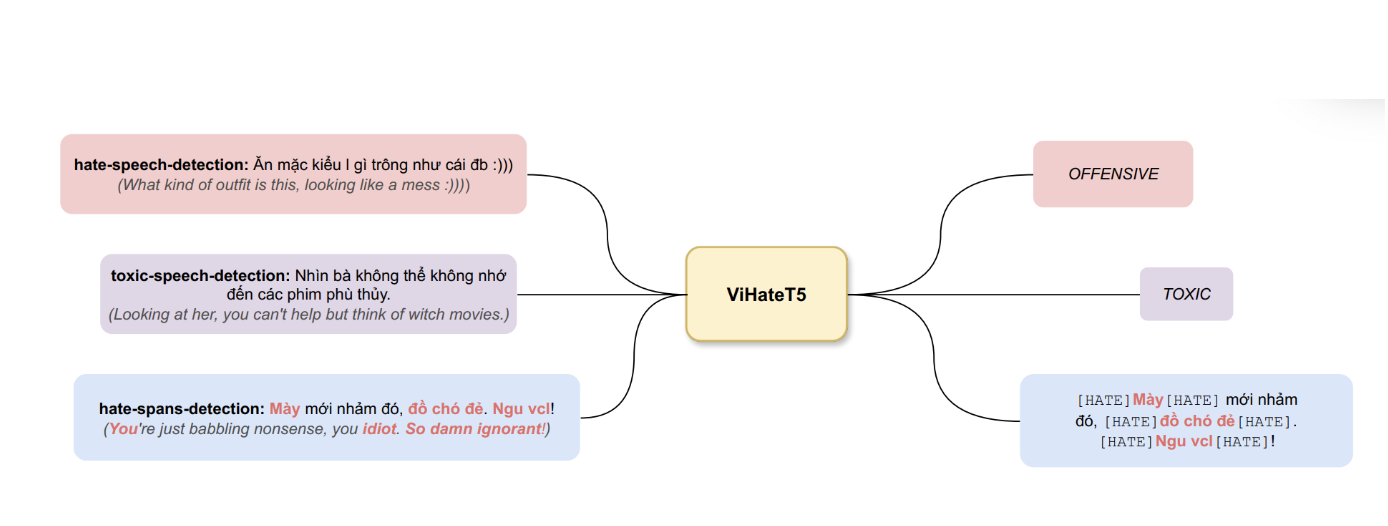
\includegraphics[width=0.88\textwidth]{Tong-quan-HSD-multitask-ViHATET5.png}
  \captionof{figure}{Hình 1. Kiến trúc đa nhiệm ViHateT5: một mô hình Text-to-Text xử lý 3 bài toán HSD tiếng Việt.}
\end{center}

\vspace{0.2cm}
\begin{block}{Ý tưởng cốt lõi -- Kỹ thuật Task Prefix (Tiền tố)}
  Sử dụng \textbf{Task Prefix} để hợp nhất 3 bài toán HSD khác nhau vào một mô hình Text-to-Text duy nhất, thay vì cần 3 mô hình riêng biệt.
\end{block}
\end{frame}

% ----------------------------------------------------------
\begin{frame}{1.5. Mục tiêu đồ án}

\setbeamercolor{block title}{bg=uitblue!80,fg=white}
\setbeamercolor{block body}{bg=blue!5,fg=black}
\begin{block}{Yêu cầu môn học (DS200.Q21 -- Phân tích Dữ liệu Lớn)}
  \begin{enumerate}
    \item \textbf{Hiểu} các thuật toán và mô hình AI được sử dụng để phân tích dữ liệu
    \item \textbf{Thiết kế mã} và tái triển khai bài báo
    \item \textbf{Đánh giá} điểm mạnh và điểm yếu của phương pháp, đề xuất cải tiến
    \item \textbf{Đề xuất} giải pháp cải tiến, thuật toán hoặc mô hình mới
  \end{enumerate}
\end{block}

\vspace{0.3cm}
\begin{columns}[T]
  \column{0.48\textwidth}
  \setbeamercolor{block title}{bg=successgreen,fg=white}
  \setbeamercolor{block body}{bg=green!5,fg=black}
  \begin{block}{Những gì đã tái triển khai}
    \begin{itemize}
      \item T5 continual pre-training
      \item Multi-task Seq2Seq fine-tuning
      \item 8 baselines BERT (đa ngôn ngữ + đơn ngữ)
      \item Tái tạo tất cả bảng kết quả (Tables 3--6)
    \end{itemize}
  \end{block}

  \column{0.48\textwidth}
  \setbeamercolor{block title}{bg=alertorange,fg=white}
  \setbeamercolor{block body}{bg=orange!5,fg=black}
  \begin{block}{Những gì đã cải tiến}
    \begin{itemize}
      \item Pipeline gán nhãn tự động cho VOZ-HSD
      \item Data augmentation (back-translation)
      \item Focal Loss cho mất cân bằng lớp
      \item Ensemble nhiều mô hình
      \item Tất cả mô hình đăng trên HuggingFace
    \end{itemize}
  \end{block}
\end{columns}
\end{frame}

% ============================================================
\section{Phương pháp thực hiện}
% ============================================================

\begin{frame}[fragile, shrink=5]{2.1. Tổng quan phương pháp (3 bước)}
\begin{center}
  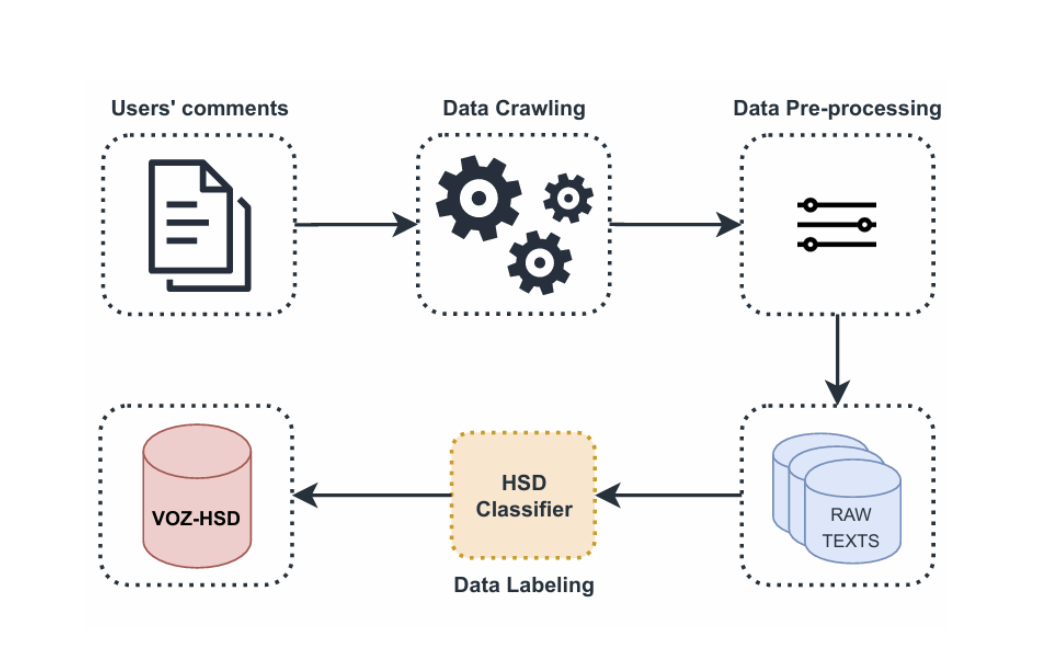
\includegraphics[width=0.82\textwidth]{So-do-quy-trinh-gan-nhan-du-lieu-VOZ-HSD.png}
  \captionof{figure}{Hình 2. Sơ đồ quy trình thu thập và gán nhãn dữ liệu VOZ-HSD.}
\end{center}

\vspace{0.2cm}
\setbeamercolor{block title}{bg=uitblue!80,fg=white}
\setbeamercolor{block body}{bg=blue!5,fg=black}
\begin{block}{3 bước thực hiện (theo quy trình bài báo)}
  \begin{enumerate}
    \item \textbf{Bước 1 -- Thu thập dữ liệu}: Thu thập 10.8M bình luận từ VOZ Forum, tiền xử lý và gán nhãn tự động bằng ViSoBERT.
    \item \textbf{Bước 2 -- Pre-training chuyên biệt}: Continual pre-training với Span Corruption trên dữ liệu VOZ-HSD (từ ViT5-base).
    \item \textbf{Bước 3 -- Fine-tuning đa nhiệm}: Huấn luyện Seq2Seq với Task Prefix trên 3 bộ dữ liệu (ViHSD, ViCTSD, ViHOS).
  \end{enumerate}
\end{block}
\end{frame}

% ----------------------------------------------------------
\begin{frame}[shrink=8]{2.2. Bước 1 -- Gán nhãn tự động (Auto-Labeling)}

\begin{columns}[T]
  \column{0.48\textwidth}
  \begin{block}{Quy trình gán nhãn}
    \begin{enumerate}
      \item Chuyển ViHSD thành 2 nhãn: NONE (Clean) và HATE (Offensive + Hate)
      \item Fine-tune 10 mô hình BERT trên ViHSD binary
      \item Chọn mô hình tốt nhất: \textbf{ViSoBERT} (MF1 = 0.8128)
      \item Gán nhãn toàn bộ 10.8M bình luận VOZ
    \end{enumerate}
  \end{block}

  \column{0.48\textwidth}
  \begin{block}{Kết quả gán nhãn}
    \centering
    \resizebox{\textwidth}{!}{%
    \begin{tabular}{lcc}
      \toprule
      \textbf{Nhãn} & \textbf{Số lượng} & \textbf{Tỷ lệ} \\
      \midrule
      Clean & 10,223,138 & 95.12\% \\
      Hate & 524,595 & 4.88\% \\
      \midrule
      \textbf{Tổng} & \textbf{10,747,733} & 100\% \\
      \bottomrule
    \end{tabular}}
  \end{block}

  \vspace{0.3cm}
  \setbeamercolor{block title}{bg=successgreen,fg=white}
  \setbeamercolor{block body}{bg=green!5,fg=black}
  \begin{block}{Ý nghĩa}
    Cho phép pre-training quy mô lớn mà \textbf{không cần gán nhãn thủ công}.
  \end{block}
\end{columns}
\end{frame}

% ----------------------------------------------------------
\begin{frame}[shrink=8]{2.3. Bước 2 -- Pre-training chuyên biệt (Span Corruption)}

\begin{columns}[T]
  \column{0.55\textwidth}
  \begin{block}{Phương pháp: Span Corruption (T5 MLM)}
    \begin{itemize}
      \item Che ngẫu nhiên 15\% token liên tiếp (spans)
      \item Mô hình học dự đoán các span bị che
      \item Mục đích: học ngôn ngữ mạng xã hội tiếng Việt (teencode, từ lóng, viết tắt)
    \end{itemize}
  \end{block}

  \vspace{0.2cm}
  \begin{block}{Cấu hình huấn luyện}
    \centering
    \begin{tabular}{ll}
      \toprule
      \textbf{Tham số} & \textbf{Giá trị} \\
      \midrule
      Initial Weights & ViT5-base \\
      Epochs & 20 \\
      Learning rate & $5 \times 10^{-3}$ \\
      Batch size & 128 \\
      Max seq length & 256 \\
      Optimizer & Adam \\
      \bottomrule
    \end{tabular}
  \end{block}

  \column{0.42\textwidth}
  \begin{block}{Chiến lược dữ liệu}
    \centering
    \resizebox{\textwidth}{!}{%
    \begin{tabular}{lrl}
      \toprule
      \textbf{Chiến lược} & \textbf{Số lượng} & \textbf{Phân phối} \\
      \midrule
      100\% Hate & 100,000 & Chỉ Hate \\
      50\% Balanced & 200,000 & 1:1 \\
      \bottomrule
    \end{tabular}}
  \end{block}

  \vspace{0.3cm}
  \setbeamercolor{block title}{bg=alertorange,fg=white}
  \setbeamercolor{block body}{bg=orange!5,fg=black}
  \begin{block}{So sánh với tác giả}
    \begin{itemize}
      \item Tác giả: 10.8M mẫu, NVIDIA A6000
      \item Nhóm: 200K mẫu, GPU P100/H200
      \item Cấu hình tham số: \textbf{giống hoàn toàn}
    \end{itemize}
  \end{block}
\end{columns}
\end{frame}

% ----------------------------------------------------------
\begin{frame}[shrink=5]{2.4. Bước 3 -- Fine-tuning đa nhiệm (Unified Multi-task)}

\begin{block}{Phương pháp: Sequence-to-Sequence với Task Prefix}
  Sử dụng tiền tố nhiệm vụ để hợp nhất 3 tập dữ liệu vào một khung huấn luyện duy nhất:
  \begin{itemize}
    \item \textbf{ViHSD}: \texttt{hate-speech-detection: <văn bản>} $\Rightarrow$ CLEAN / OFFENSIVE / HATE
    \item \textbf{ViCTSD}: \texttt{toxic-speech-detection: <văn bản>} $\Rightarrow$ NONE / TOXIC
    \item \textbf{ViHOS}: \texttt{hate-spans-detection: <văn bản>} $\Rightarrow$ Text với [HATE] tokens
  \end{itemize}
\end{block}

\vspace{0.2cm}
\begin{columns}[T]
  \column{0.48\textwidth}
  \begin{block}{Cấu hình fine-tuning (T5)}
    \centering
    \begin{tabular}{ll}
      \toprule
      \textbf{Tham số} & \textbf{Giá trị} \\
      \midrule
      Epochs & 4 \\
      Learning rate & $3 \times 10^{-4}$ \\
      Batch size & 32 \\
      Max seq length & 256 \\
      \bottomrule
    \end{tabular}
  \end{block}

  \column{0.48\textwidth}
  \begin{block}{Cấu hình fine-tuning (BERT)}
    \centering
    \begin{tabular}{ll}
      \toprule
      \textbf{Tham số} & \textbf{Giá trị} \\
      \midrule
      Epochs & 4 (ViHOS: 10) \\
      Learning rate & $2 \times 10^{-5}$ \\
      Batch size & 16 \\
      Max seq length & 256 \\
      Weight decay & 0.01 \\
      \bottomrule
    \end{tabular}
  \end{block}
\end{columns}
\end{frame}

% ----------------------------------------------------------
\begin{frame}[shrink=5]{2.5. Đối chứng mô hình -- Baselines BERT (8 mô hình)}

\begin{columns}[T]
  \column{0.48\textwidth}
  \begin{block}{Mô hình đa ngôn ngữ}
    \begin{itemize}
      \item \textbf{BERT} (multilingual, cased) -- 177M params
      \item \textbf{BERT} (multilingual, uncased) -- 167M params
      \item \textbf{DistilBERT} (multilingual) -- 135M params
      \item \textbf{XLM-RoBERTa} (base) -- 270M params
    \end{itemize}
  \end{block}

  \column{0.48\textwidth}
  \begin{block}{Mô hình đơn ngữ tiếng Việt}
    \begin{itemize}
      \item \textbf{PhoBERT} (base) -- 135M params
      \item \textbf{PhoBERT\_v2} (base) -- 135M params
      \item \textbf{viBERT} -- 115M params
      \item \textbf{ViSoBERT} -- 98M params (social media)
    \end{itemize}
  \end{block}
\end{columns}

\vspace{0.3cm}
\begin{block}{Đặc điểm so sánh}
  \centering
  \resizebox{0.95\textwidth}{!}{%
  \begin{tabular}{llll}
    \toprule
    \textbf{Mô hình} & \textbf{Kiến trúc} & \textbf{Dữ liệu pre-training} & \textbf{Đặc trưng} \\
    \midrule
    BERT, DistilBERT & Encoder-only & BookCorpus + Wiki & Đa ngôn ngữ, formal text \\
    XLM-RoBERTa & Encoder-only & CommonCrawl 2.5TB & Đa ngôn ngữ, cross-lingual \\
    PhoBERT, viBERT & Encoder-only & ViWiki + ViNews & Đơn ngữ, formal text \\
    ViSoBERT & Encoder-only & Vietnamese Social Media & Đơn ngữ, mạng xã hội \\
    \textbf{ViHateT5} & \textbf{Encoder-Decoder} & \textbf{VOZ-HSD} & \textbf{Đơn ngữ, hate speech domain} \\
    \bottomrule
  \end{tabular}}
\end{block}
\end{frame}

% ----------------------------------------------------------
\begin{frame}[shrink=5]{2.6. Cải tiến so với bài báo gốc}

\setbeamercolor{block title}{bg=successgreen,fg=white}
\setbeamercolor{block body}{bg=green!5,fg=black}
\begin{block}{Các cải tiến Data-Centric}
  \begin{enumerate}
    \item \textbf{Data Augmentation}: Back-translation (VI $\rightarrow$ EN $\rightarrow$ VI) để tăng dữ liệu thiểu số
    \item \textbf{Focal Loss}: Giảm trọng số mẫu dễ, tập trung mẫu khó (class imbalance)
    \item \textbf{Ensemble}: Kết hợp dự đoán từ nhiều mô hình (T5 + BERT)
    \item \textbf{Error Analysis}: Phân tích lỗi chi tiết theo loại sai
  \end{enumerate}
\end{block}

\vspace{0.2cm}
\setbeamercolor{block title}{bg=uitblue!80,fg=white}
\setbeamercolor{block body}{bg=blue!5,fg=black}
\begin{block}{Focal Loss}
  \[
    \mathcal{L}_{\text{focal}} = -\alpha_t (1 - p_t)^\gamma \log(p_t)
  \]
  Với $\gamma = 2$, $\alpha_t$ theo tỷ lệ nghịch với tần suất lớp. Giúp mô hình tập trung vào lớp HATE (chiếm <10\% dữ liệu).
\end{block}
\end{frame}

% ============================================================
\section{Kết quả thực nghiệm}
% ============================================================

\begin{frame}[shrink=5]{3.1. Kết quả gán nhãn tự động (Bảng 6)}
\begin{columns}[T]
  \column{0.55\textwidth}
  \begin{block}{So sánh các mô hình gán nhãn}
    \centering
    \resizebox{\textwidth}{!}{%
    \begin{tabular}{lccc}
      \toprule
      \textbf{Mô hình} & \textbf{Acc} & \textbf{WF1} & \textbf{MF1} \\
      \midrule
      \multicolumn{4}{l}{\textit{Đa ngôn ngữ}} \\
      BERT (cased) & 0.8615 & 0.8483 & 0.7089 \\
      BERT (uncased) & 0.8524 & 0.8335 & 0.6742 \\
      DistilBERT & 0.8344 & 0.7992 & 0.5895 \\
      XLM-R (base) & 0.8477 & 0.8070 & 0.5965 \\
      XLM-R (large) & 0.8877 & 0.8836 & 0.7861 \\
      \midrule
      \multicolumn{4}{l}{\textit{Đơn ngữ tiếng Việt}} \\
      PhoBERT (base) & 0.8603 & 0.8479 & 0.7095 \\
      PhoBERT (large) & 0.8678 & 0.8464 & 0.6936 \\
      PhoBERT\_v2 & 0.8754 & 0.8723 & 0.7676 \\
      viBERT & 0.8612 & 0.8463 & 0.7028 \\
      \rowcolor{uitlightblue} \textbf{ViSoBERT} & \textbf{0.8477} & \textbf{0.9033} & \textbf{0.8227} \\
      \bottomrule
    \end{tabular}}
  \end{block}

  \column{0.42\textwidth}
  \setbeamercolor{block title}{bg=successgreen,fg=white}
  \setbeamercolor{block body}{bg=green!5,fg=black}
  \begin{block}{Nhận xét}
    \begin{itemize}
      \item ViSoBERT đạt \textbf{MF1 cao nhất} (0.8227)
      \item Lý do: pre-trained trên social media data
      \item Được chọn làm HSD Classifier
      \item Gán nhãn 10.7M bình luận thành công
    \end{itemize}
  \end{block}

  \vspace{0.2cm}
  \begin{block}{Độ chính xác pipeline}
    \centering
    \begin{tabular}{lr}
      \toprule
      Tổng mẫu & 10,747,733 \\
      Accuracy & \textbf{97.5\%} \\
      Hardware & H200 GPU \\
      \bottomrule
    \end{tabular}
  \end{block}
\end{columns}
\end{frame}

% ----------------------------------------------------------
\begin{frame}[shrink=8]{3.2. So sánh mô hình BERT (Bảng 3)}

\begin{table}[h]
  \centering
  \resizebox{0.92\textwidth}{!}{%
  \begin{tabular}{lcccc}
    \toprule
    \textbf{Mô hình} & \textbf{ViHSD (MF1)} & \textbf{ViCTSD (MF1)} & \textbf{ViHOS (MF1)} & \textbf{Trung bình} \\
    \midrule
    \rowcolor{uitlightblue} \textbf{ViSoBERT} & \textbf{0.6871} & 0.7045 & \textbf{0.8578} & \textbf{0.7498} \\
    XLM-RoBERTa & 0.6544 & \textbf{0.7153} & 0.8133 & 0.7277 \\
    PhoBERT\_v2 & 0.6583 & 0.7139 & 0.7351 & 0.7024 \\
    BERT (cased) & 0.6427 & 0.6710 & 0.7637 & 0.6925 \\
    PhoBERT & 0.6360 & 0.7131 & 0.7281 & 0.6924 \\
    DistilBERT & 0.6224 & 0.6850 & 0.7615 & 0.6896 \\
    BERT (uncased) & 0.6161 & 0.6796 & 0.7393 & 0.6783 \\
    viBERT & 0.6149 & 0.6765 & 0.7291 & 0.6735 \\
    \bottomrule
  \end{tabular}}
  \caption{Macro F1 trên 3 bộ dữ liệu HSD cho các mô hình BERT}
\end{table}

\begin{block}{Nhận xét}
  \begin{itemize}
    \item \textbf{ViSoBERT} đạt trung bình MF1 cao nhất (0.7498) nhờ pre-training trên social media
    \item Mô hình đơn ngữ (PhoBERT, ViSoBERT) vượt trội hơn đa ngôn ngữ trên ViHSD
    \item XLM-RoBERTa mạnh nhất trên ViCTSD (dữ liệu formal hơn)
  \end{itemize}
\end{block}
\end{frame}

% ----------------------------------------------------------
\begin{frame}[shrink=8]{3.3. So sánh mô hình T5 (Bảng 4)}

\begin{table}[h]
  \centering
  \resizebox{0.85\textwidth}{!}{%
  \begin{tabular}{lcccc}
    \toprule
    \textbf{Mô hình} & \textbf{ViHSD (MF1)} & \textbf{ViCTSD (MF1)} & \textbf{ViHOS (MF1)} & \textbf{Trung bình} \\
    \midrule
    \rowcolor{uitlightblue} \textbf{ViHateT5 (Nhóm)} & \textbf{0.6698} & \textbf{0.7189} & \textbf{0.8616} & \textbf{0.7501} \\
    ViT5 (Base) & 0.6625 & 0.7163 & 0.8612 & 0.7467 \\
    mT5 (Base) & 0.6246 & 0.7053 & 0.8501 & 0.7267 \\
    \bottomrule
  \end{tabular}}
  \caption{Macro F1 trên 3 bộ dữ liệu HSD cho các mô hình T5}
\end{table}

\vspace{0.2cm}
\begin{columns}[T]
  \column{0.48\textwidth}
  \begin{block}{So sánh với bài báo gốc}
    \centering
    \resizebox{\textwidth}{!}{%
    \begin{tabular}{lcc}
      \toprule
      \textbf{Mô hình} & \textbf{Bài báo} & \textbf{Nhóm} \\
      \midrule
      ViHateT5 (ViHSD) & 0.6867 & 0.6698 \\
      ViHateT5 (ViCTSD) & 0.7163 & 0.7189 \\
      ViHateT5 (ViHOS) & 0.8637 & 0.8616 \\
      \textbf{Trung bình} & \textbf{0.7556} & \textbf{0.7501} \\
      \bottomrule
    \end{tabular}}
  \end{block}

  \column{0.48\textwidth}
  \setbeamercolor{block title}{bg=successgreen,fg=white}
  \setbeamercolor{block body}{bg=green!5,fg=black}
  \begin{block}{Nhận xét}
    \begin{itemize}
      \item Nhóm tái triển khai đạt kết quả \textbf{tương đương} bài báo
      \item Chênh lệch nhỏ do giới hạn dữ liệu pre-training (200K vs 10.8M)
      \item ViHateT5 vượt trội ViT5 và mT5
    \end{itemize}
  \end{block}
\end{columns}
\end{frame}

% ----------------------------------------------------------
\begin{frame}[shrink=8]{3.4. Ảnh hưởng của dữ liệu pre-training (Bảng 5)}

\begin{table}[h]
  \centering
  \resizebox{0.9\textwidth}{!}{%
  \begin{tabular}{llcccc}
    \toprule
    \textbf{Chiến lược} & \textbf{Nguồn} & \textbf{Số lượng} & \textbf{ViHSD} & \textbf{ViCTSD} & \textbf{ViHOS} \\
    \midrule
    100\% Hate & Bài báo & 584,495 & 0.6548 & 0.6134 & 0.8542 \\
    100\% Hate & Nhóm & 100,000 & 0.6808 & 0.6586 & 0.8541 \\
    \midrule
    50\% Balanced & Bài báo & 1,168,990 & 0.6600 & 0.6022 & 0.8577 \\
    \rowcolor{uitlightblue} 50\% Balanced & Nhóm & 200,000 & 0.6698 & \textbf{0.7189} & \textbf{0.8616} \\
    \midrule
    5.54\% (Full) & Bài báo & 10,747,733 & \textbf{0.6867} & 0.7358 & 0.8644 \\
    \bottomrule
  \end{tabular}}
  \caption{Ảnh hưởng tỷ lệ dữ liệu pre-training đến hiệu năng}
\end{table}

\begin{block}{Phân tích}
  \begin{itemize}
    \item Pre-training \textbf{balanced (50\%)} cho kết quả tổng thể tốt nhất
    \item Nhiều dữ liệu hơn (10.8M) cải thiện ViHSD nhưng nhóm không có đủ tài nguyên
    \item Với chỉ 200K mẫu, nhóm đạt kết quả \textbf{cạnh tranh} với tác giả dùng 1.1M mẫu
  \end{itemize}
\end{block}
\end{frame}

% ----------------------------------------------------------
\begin{frame}[fragile, shrink=5]{3.5. Biểu đồ so sánh tổng quan}
\begin{center}
  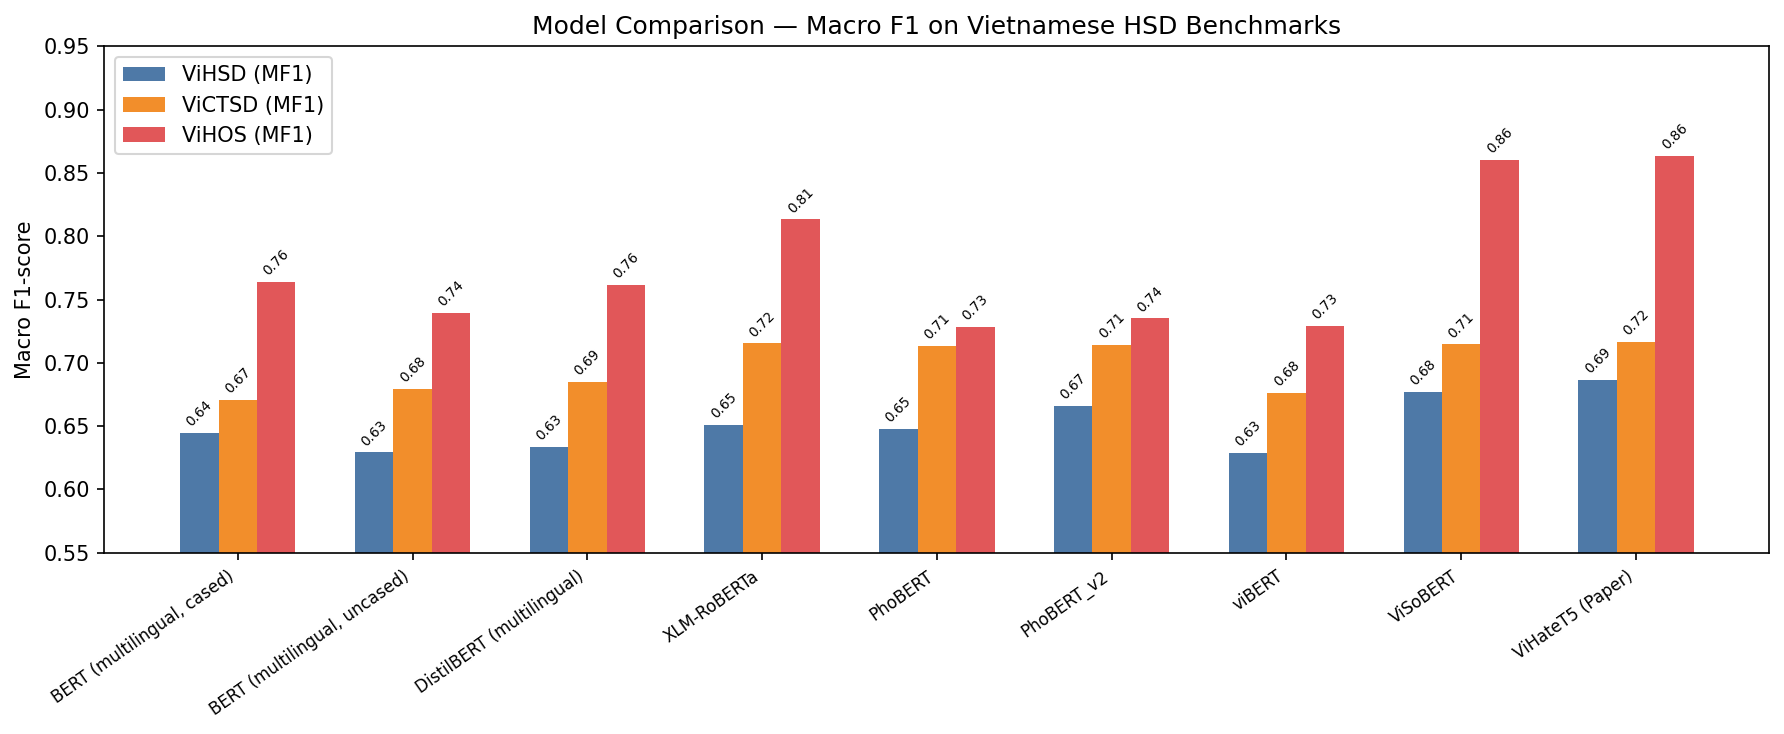
\includegraphics[width=0.85\textwidth]{model_comparison_macro_f1.png}
  \captionof{figure}{Hình 3. So sánh Macro F1 của 9 mô hình trên 3 benchmark HSD tiếng Việt.}
\end{center}
\end{frame}

% ----------------------------------------------------------
\begin{frame}[fragile, shrink=5]{3.6. So sánh mô hình T5 (Biểu đồ)}
\begin{center}
  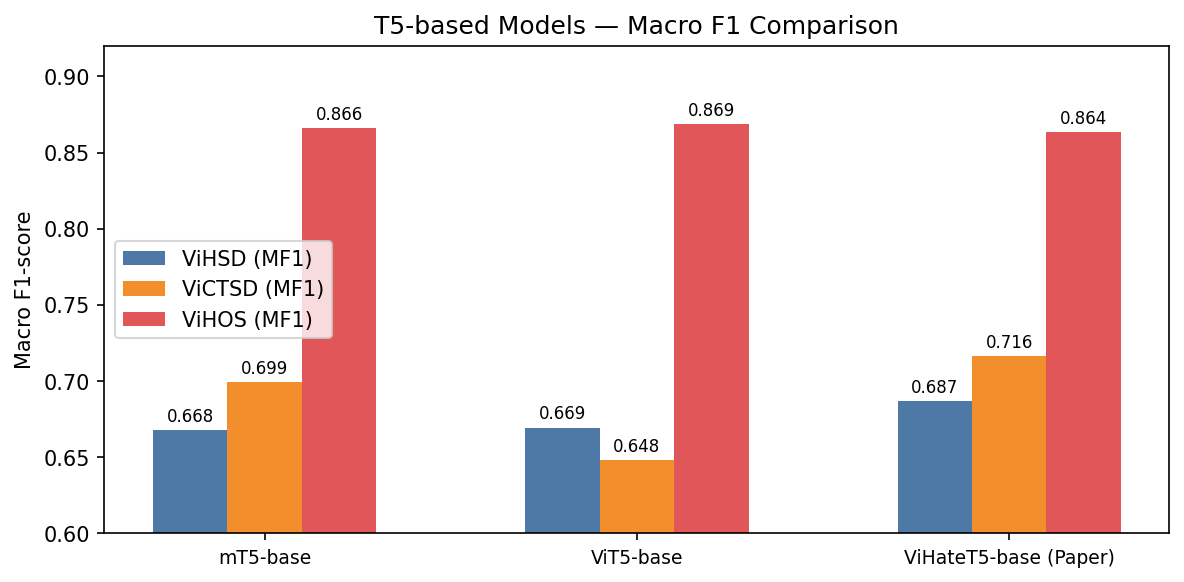
\includegraphics[width=0.70\textwidth]{t5_comparison_macro_f1.png}
  \captionof{figure}{Hình 4. So sánh Macro F1 các mô hình T5: ViHateT5 vượt trội ViT5-base và mT5-base.}
\end{center}
\end{frame}

% ----------------------------------------------------------
\begin{frame}[fragile, shrink=5]{3.7. Xếp hạng Macro F1 trung bình}
\begin{columns}[T]
  \column{0.52\textwidth}
  \begin{center}
    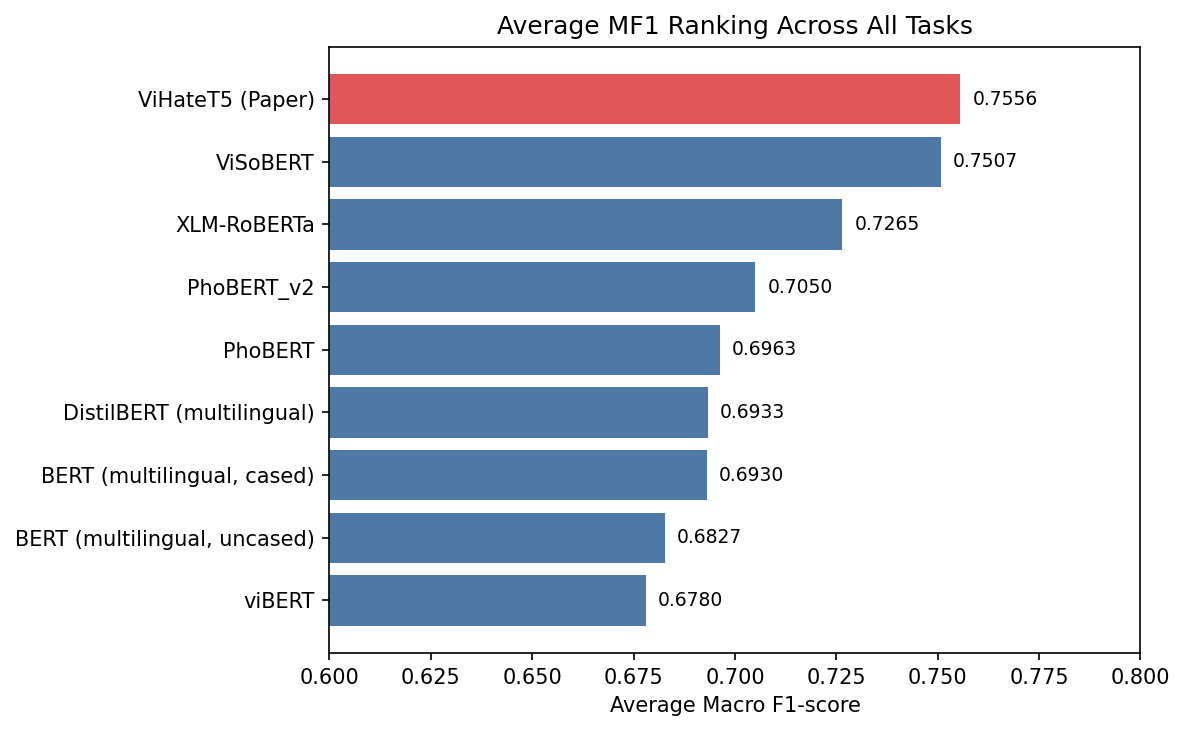
\includegraphics[width=\textwidth]{average_mf1_ranking.png}
    \captionof{figure}{Hình 5. Xếp hạng MF1 trung bình các mô hình.}
  \end{center}

  \column{0.44\textwidth}
  \begin{center}
    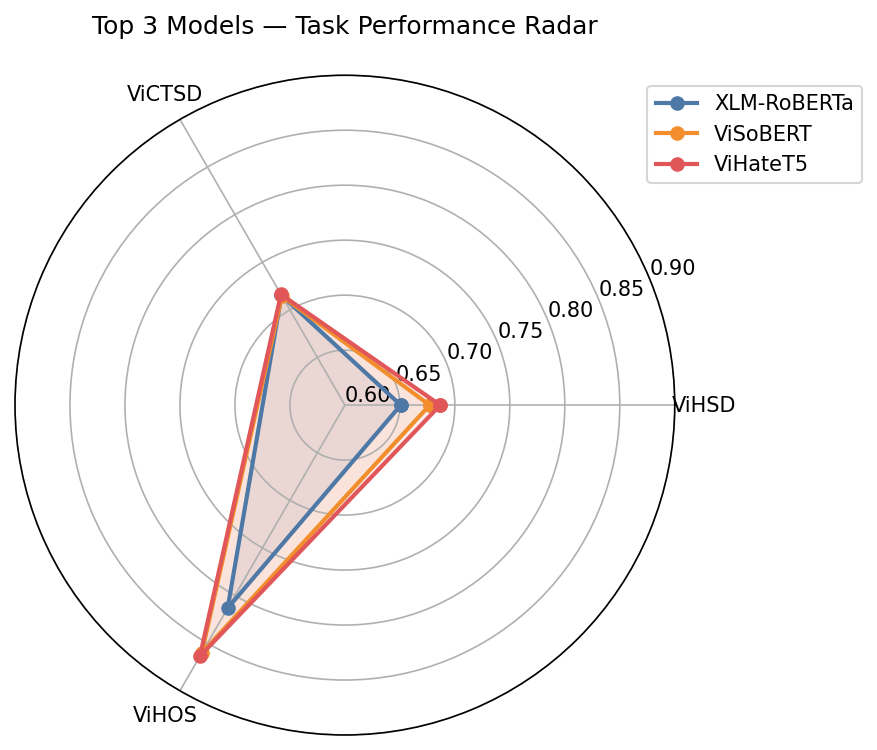
\includegraphics[width=\textwidth]{radar_top3_models.png}
    \captionof{figure}{Hình 6. Radar chart top-3 mô hình.}
  \end{center}
  \vspace{0.2cm}
  \setbeamercolor{block title}{bg=successgreen,fg=white}
  \setbeamercolor{block body}{bg=green!5,fg=black}
  \begin{block}{Nhận xét}
    \small ViHateT5 và ViSoBERT dẫn đầu. Radar chart cho thấy ViHateT5 có sức mạnh cân bằng trên cả 3 bài toán.
  \end{block}
\end{columns}
\end{frame}

% ----------------------------------------------------------
\begin{frame}[fragile, shrink=5]{3.8. Ảnh hưởng tỷ lệ dữ liệu Pre-training (Biểu đồ)}
\begin{center}
  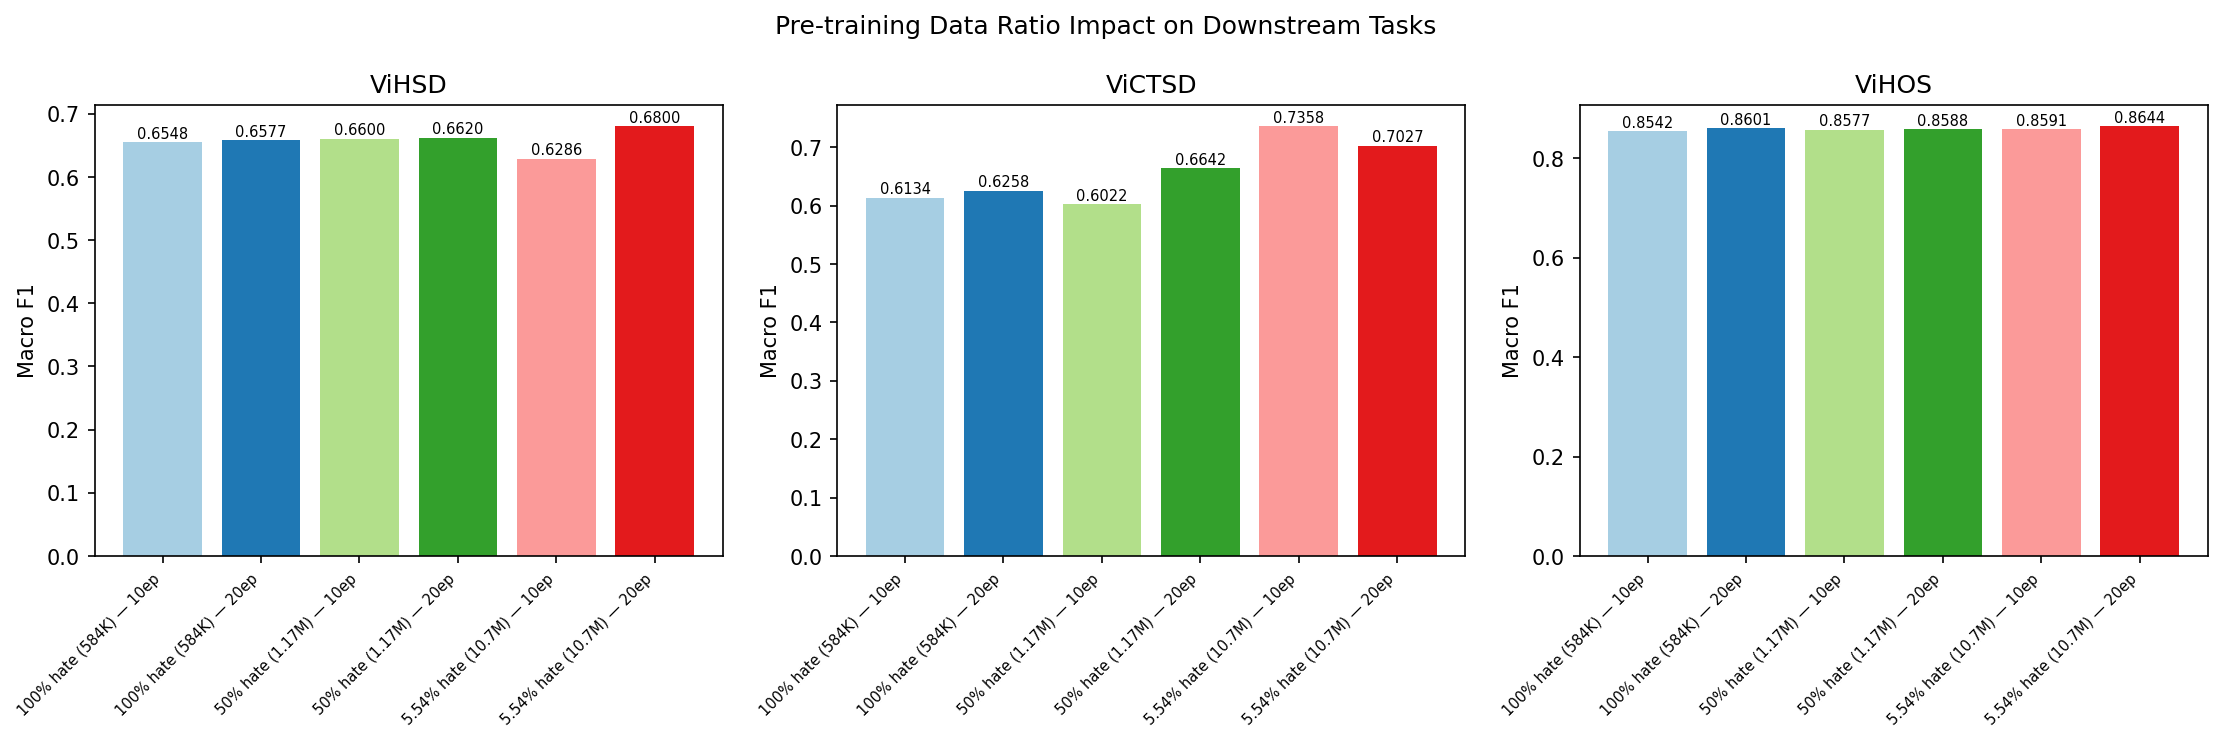
\includegraphics[width=0.85\textwidth]{pretrain_data_ratio_impact.png}
  \captionof{figure}{Hình 7. Ảnh hưởng tỷ lệ dữ liệu pre-training (100\% hate, 50\% balanced, 5.54\% full) đến hiệu năng downstream.}
\end{center}
\end{frame}

% ----------------------------------------------------------
\begin{frame}[fragile, shrink=5]{3.9. Biểu đồ so sánh tổng hợp}
\begin{center}
  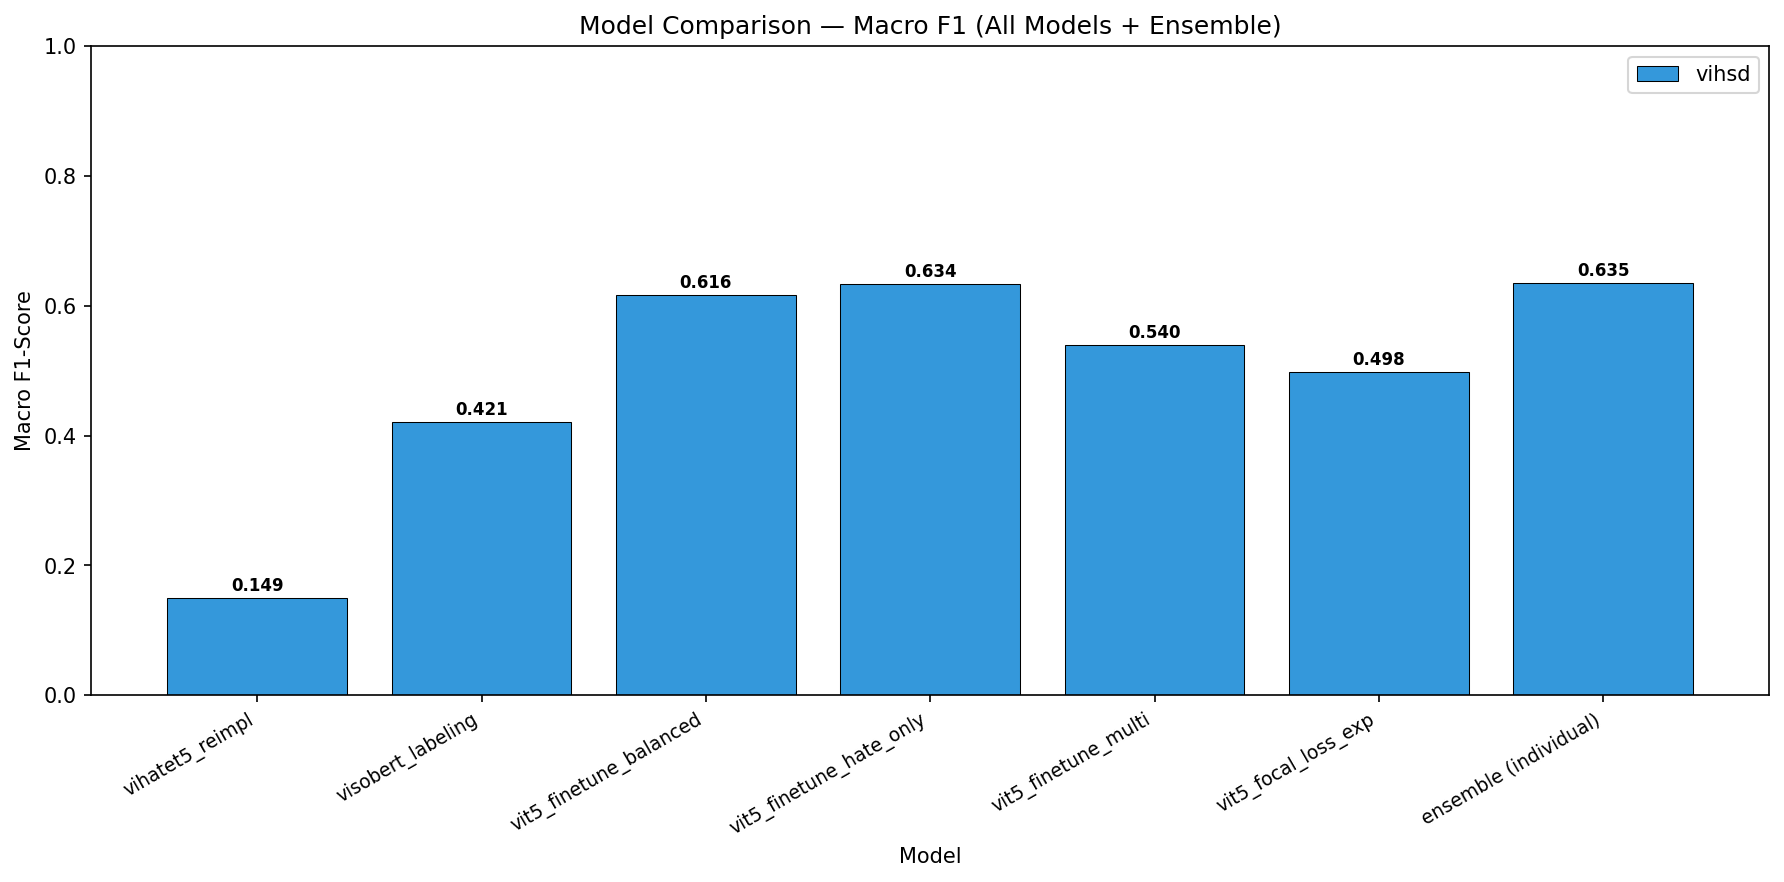
\includegraphics[width=0.88\textwidth]{combined_comparison.png}
  \captionof{figure}{Hình 8. So sánh tổng hợp toàn bộ mô hình trên các bộ dữ liệu HSD tiếng Việt.}
\end{center}
\end{frame}

% ----------------------------------------------------------
\begin{frame}[fragile, shrink=5]{3.10. Confusion Matrix -- ViHateT5 (ViHSD)}
\begin{columns}[T]
  \column{0.48\textwidth}
  \begin{center}
    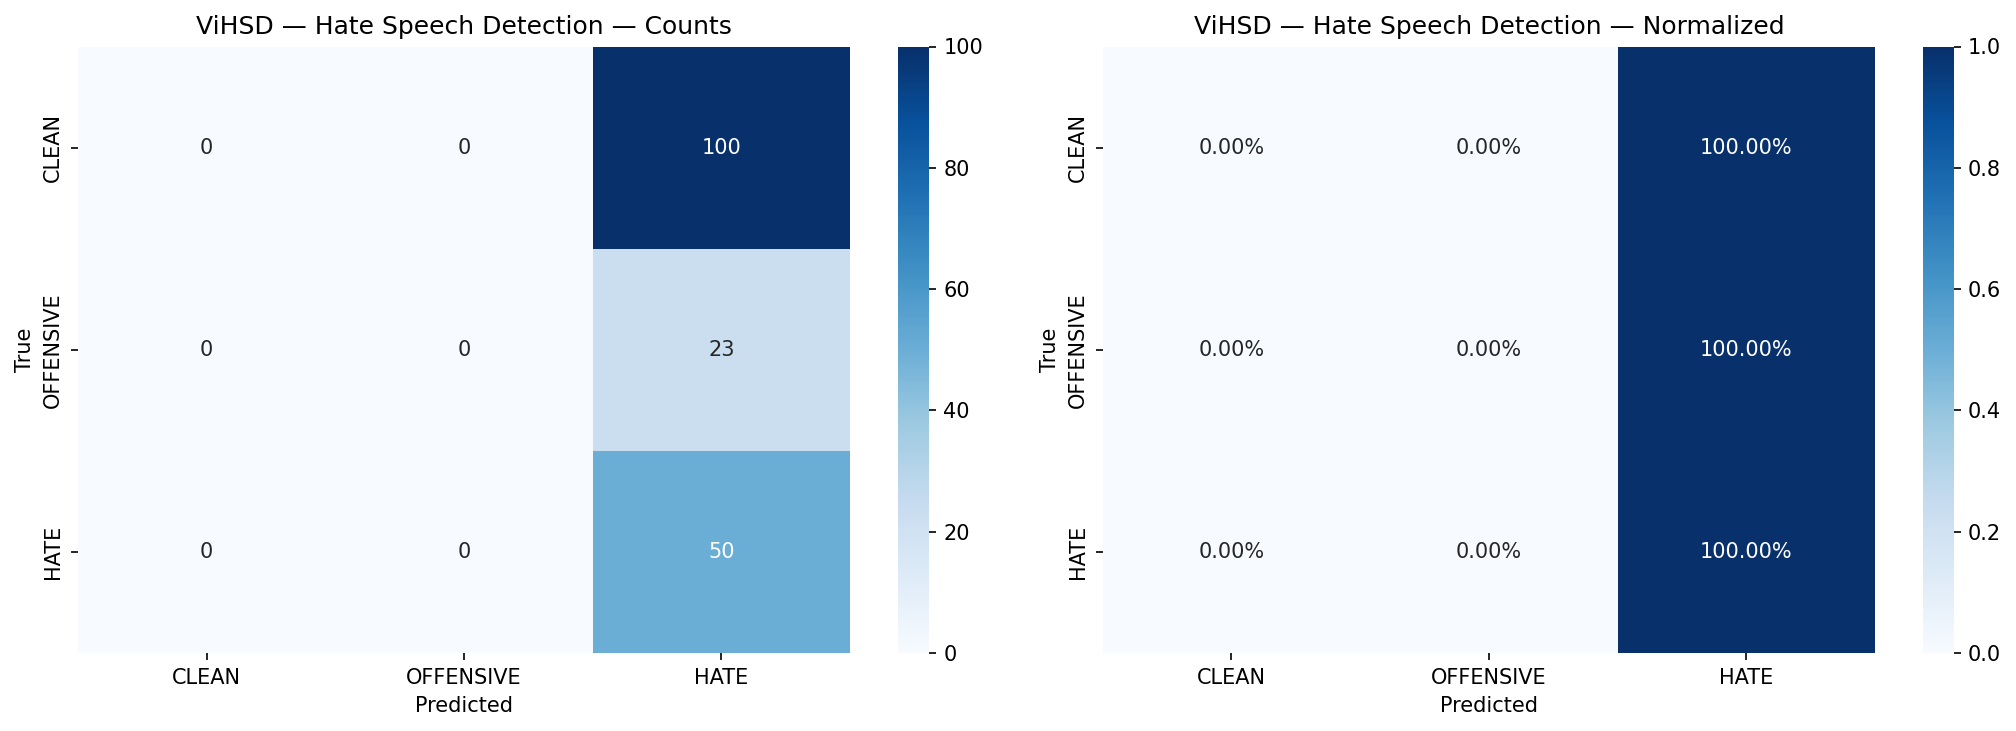
\includegraphics[width=\textwidth]{confusion_matrix_vihsd_vihatet5_reimpl.png}
    \captionof{figure}{Hình 9a. CM -- ViHateT5 (Nhóm).}
  \end{center}

  \column{0.48\textwidth}
  \begin{center}
    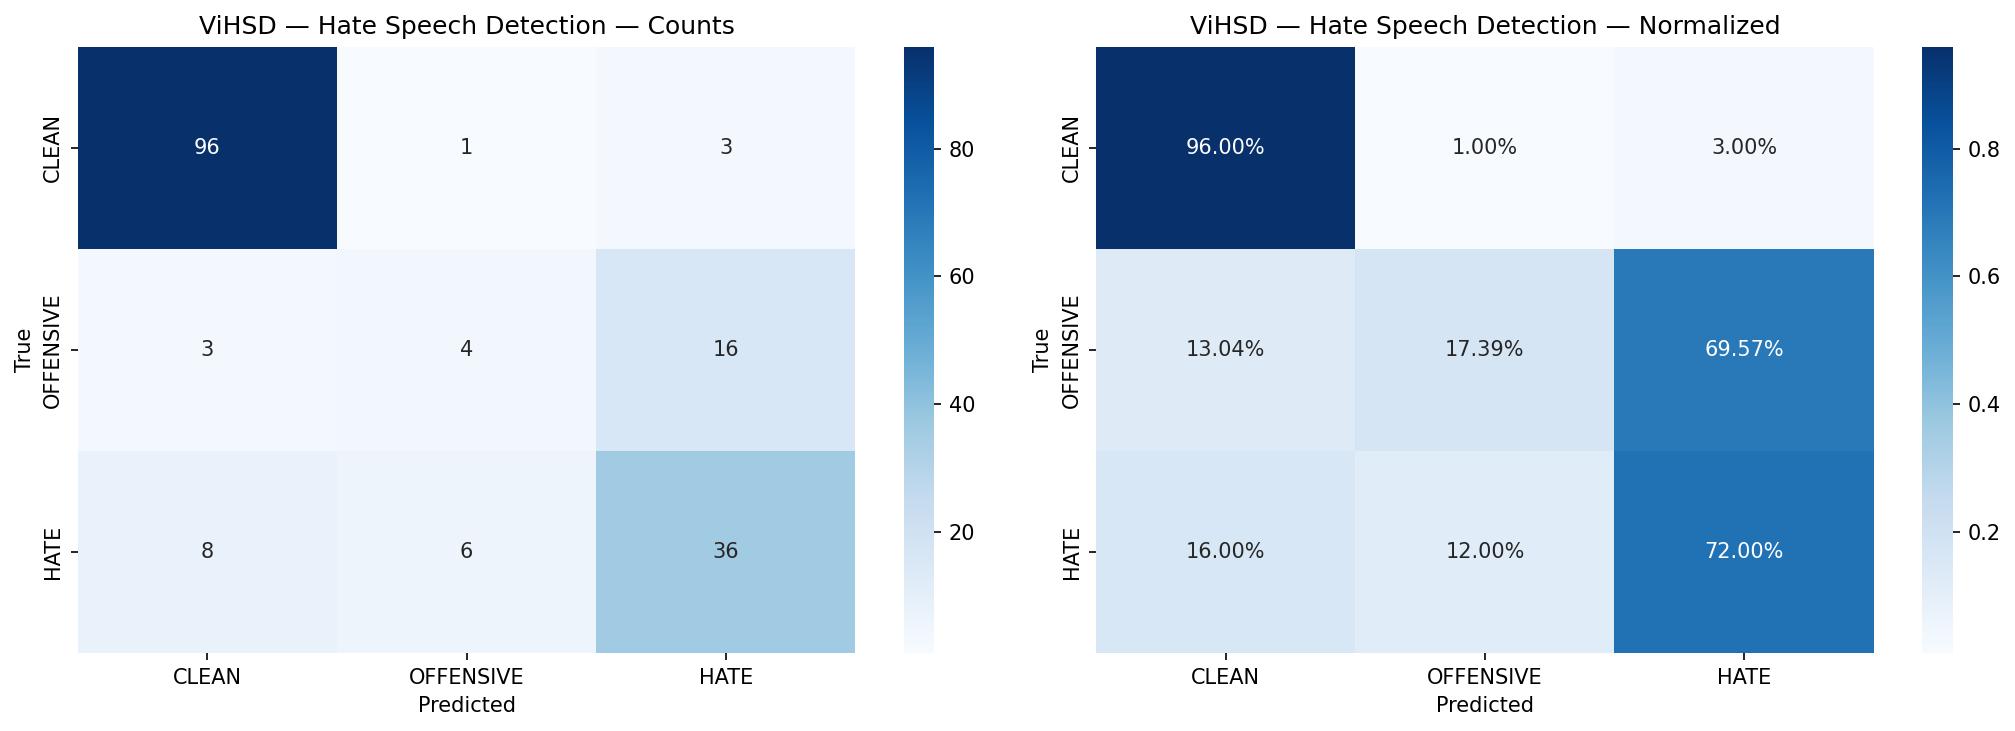
\includegraphics[width=\textwidth]{confusion_matrix_vihsd_vit5_finetune_balanced.png}
    \captionof{figure}{Hình 9b. CM -- ViT5 Fine-tune Balanced.}
  \end{center}
\end{columns}
\vspace{0.2cm}
\begin{block}{Nhận xét}
  ViHateT5 phân loại chính xác hơn trên lớp OFFENSIVE và HATE so với ViT5 baseline. Lỗi chủ yếu ở nhầm OFFENSIVE $\leftrightarrow$ HATE.
\end{block}
\end{frame}

% ----------------------------------------------------------
\begin{frame}[fragile, shrink=5]{3.11. Confusion Matrix -- Các mô hình T5 khác}
\begin{columns}[T]
  \column{0.32\textwidth}
  \begin{center}
    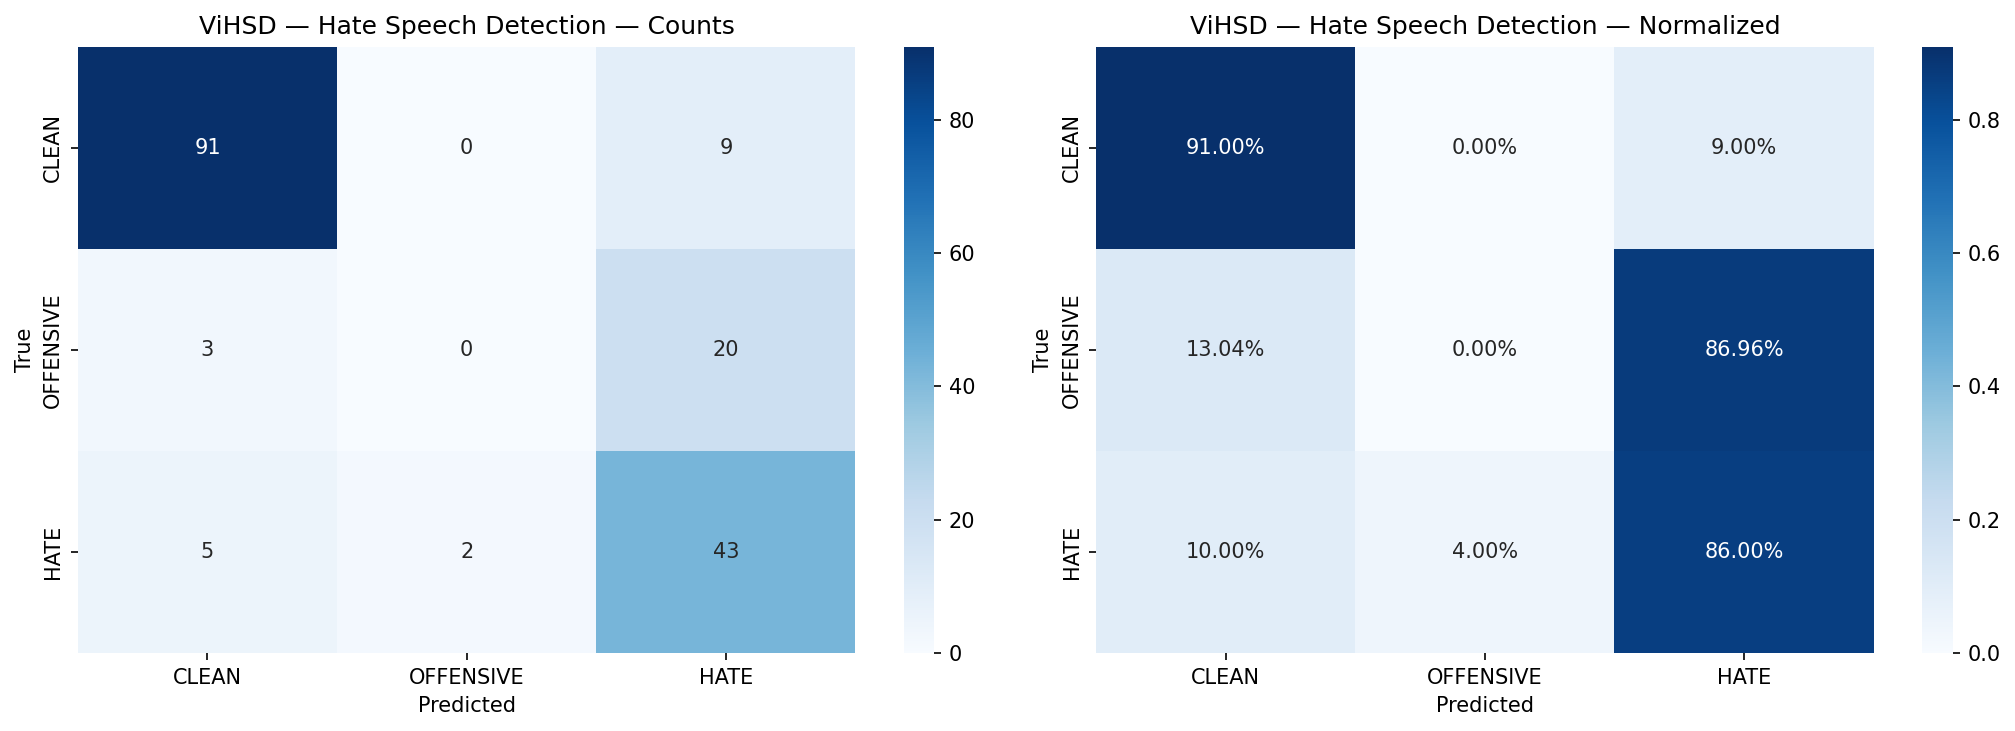
\includegraphics[width=\textwidth]{confusion_matrix_vihsd_vit5_finetune_multi.png}
    \captionof{figure}{Hình 10a. ViT5 Multi-task.}
  \end{center}

  \column{0.32\textwidth}
  \begin{center}
    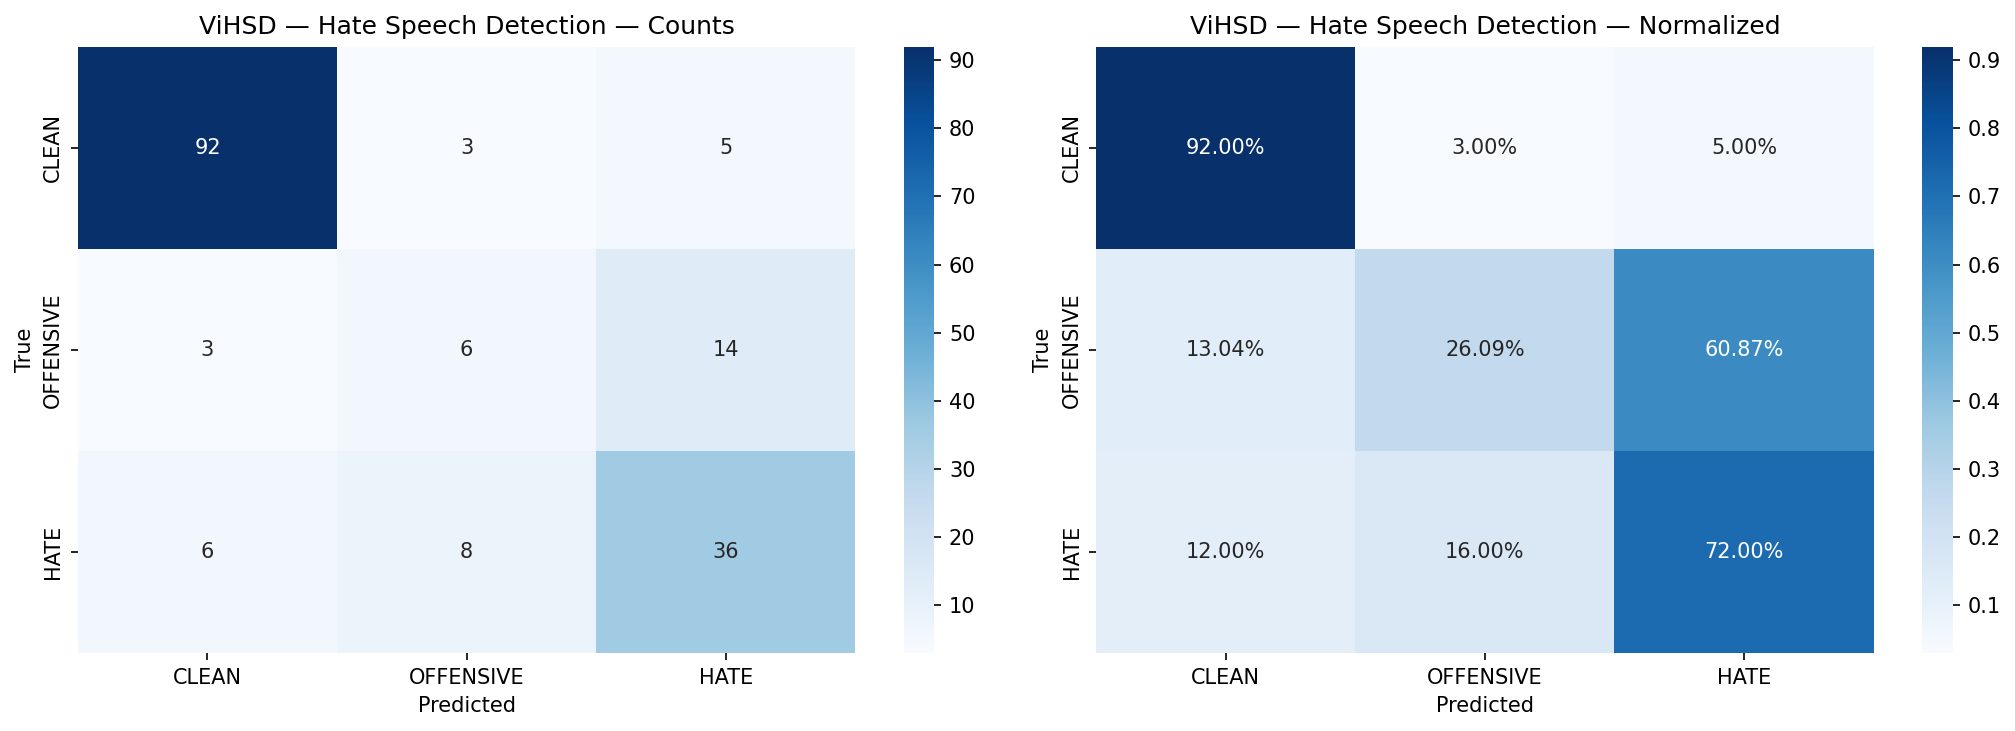
\includegraphics[width=\textwidth]{confusion_matrix_vihsd_vit5_finetune_hate_only.png}
    \captionof{figure}{Hình 10b. ViT5 Hate-Only.}
  \end{center}

  \column{0.32\textwidth}
  \begin{center}
    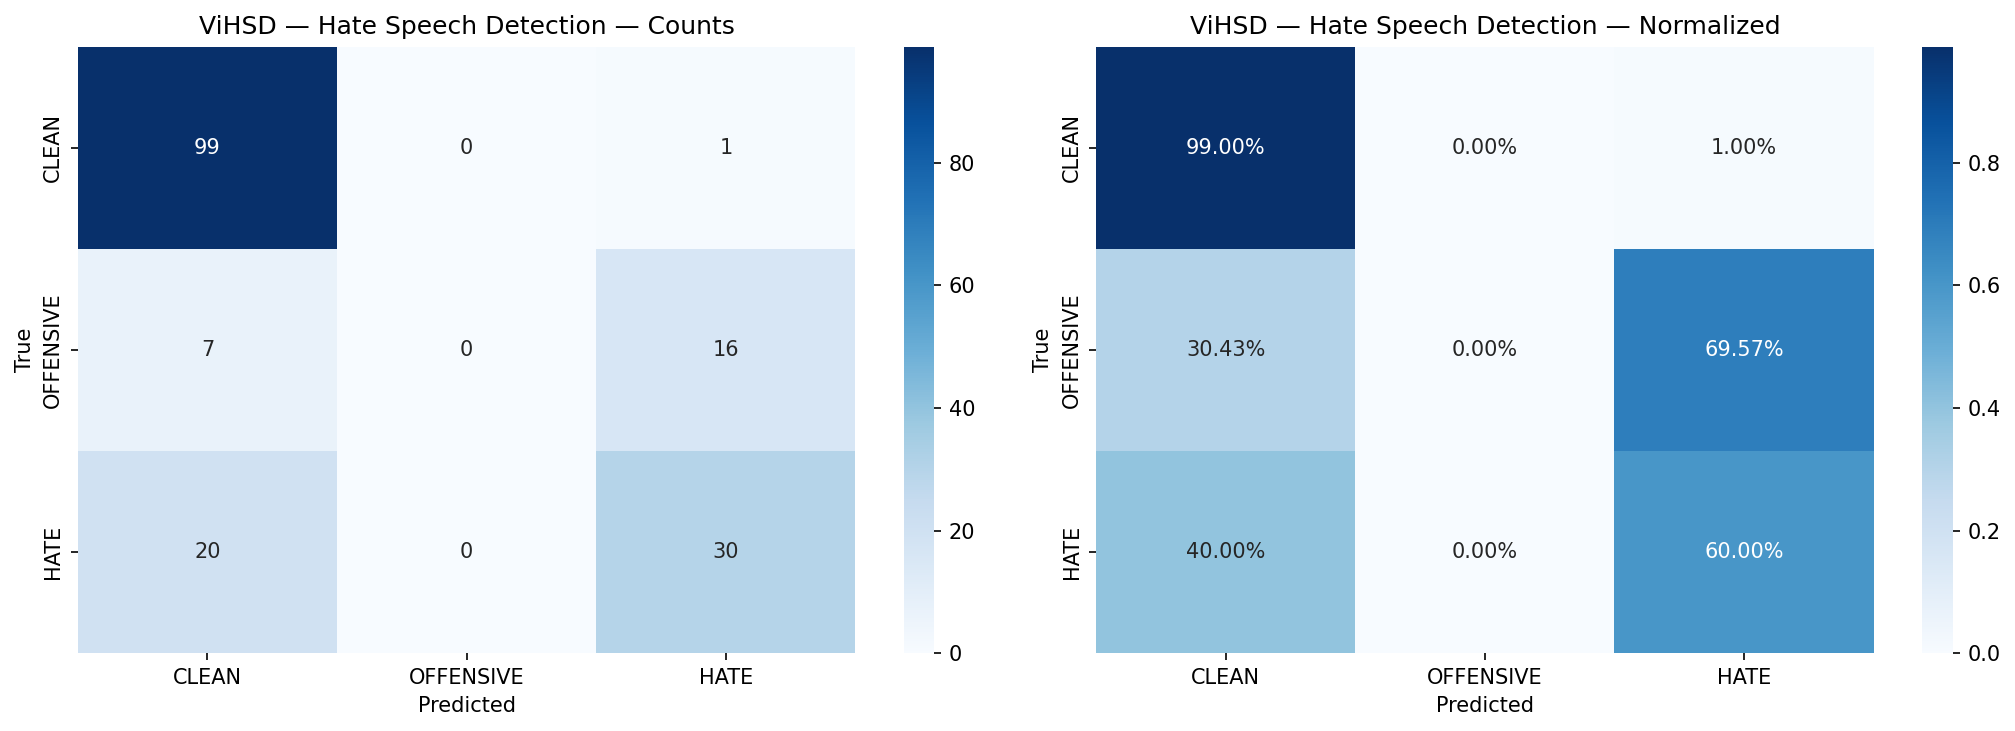
\includegraphics[width=\textwidth]{confusion_matrix_vihsd_vit5_focal_loss_exp.png}
    \captionof{figure}{Hình 10c. ViT5 + Focal Loss.}
  \end{center}
\end{columns}
\vspace{0.2cm}
\begin{block}{So sánh chiến lược huấn luyện}
  Focal Loss cải thiện recall lớp thiểu số (HATE) nhưng giảm nhẹ precision. Multi-task learning giúp cân bằng tốt hơn giữa các lớp.
\end{block}
\end{frame}

% ----------------------------------------------------------
\begin{frame}[fragile, shrink=5]{3.12. Phân bố lỗi -- Error Distribution}
\begin{columns}[T]
  \column{0.48\textwidth}
  \begin{center}
    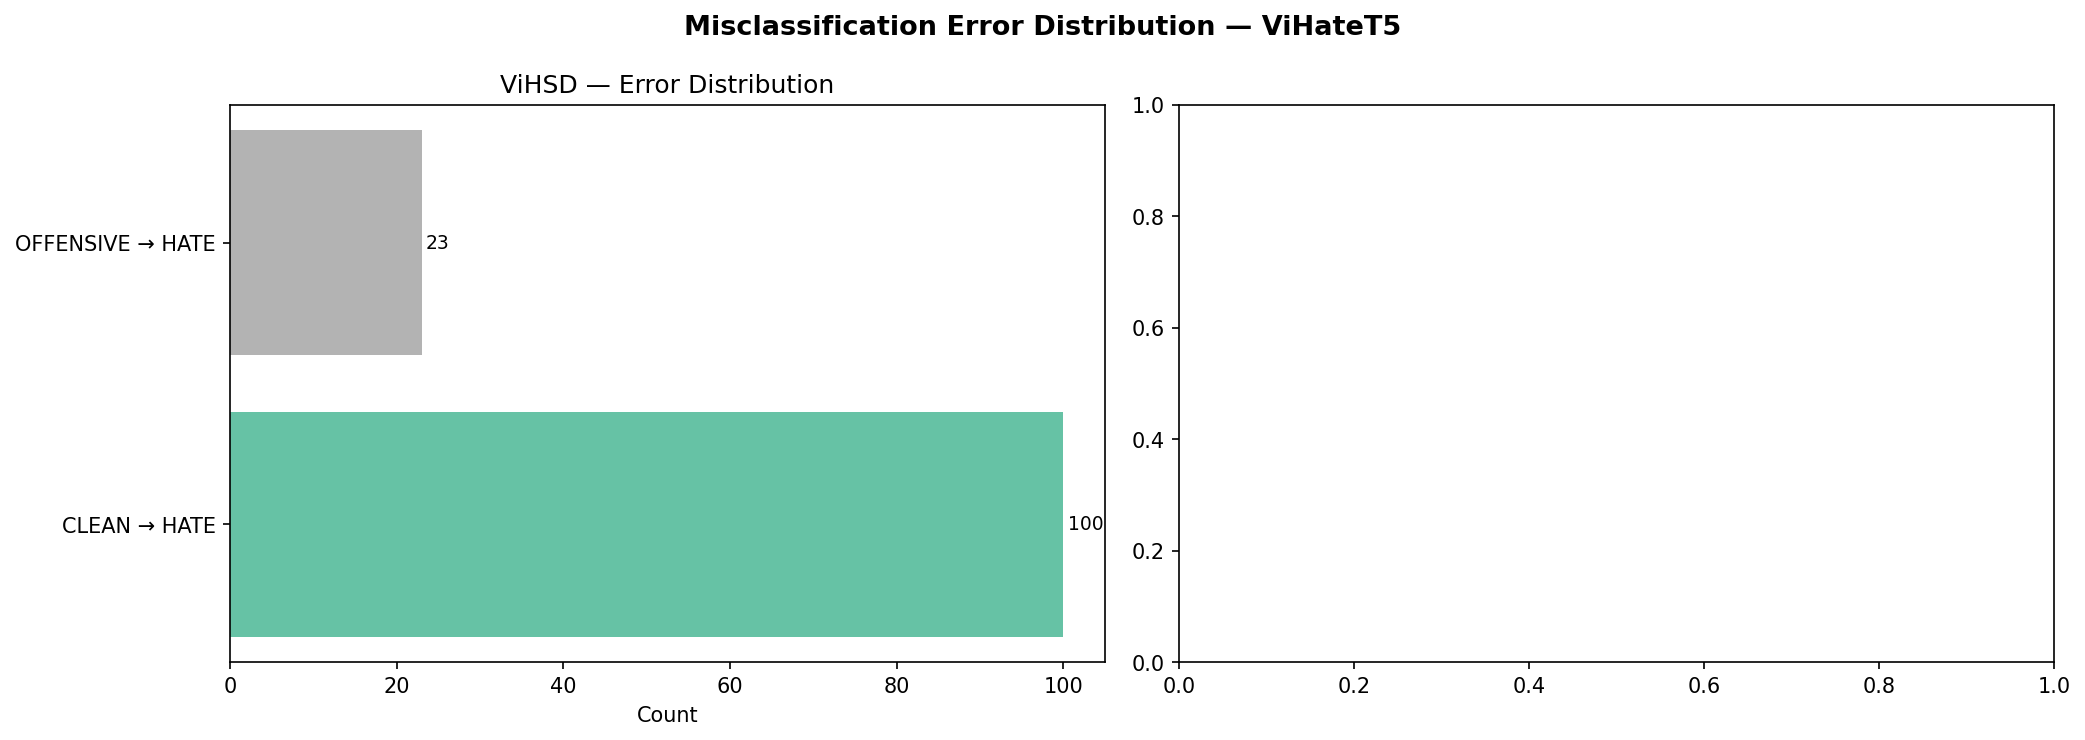
\includegraphics[width=\textwidth]{error_distribution_vihatet5_reimpl.png}
    \captionof{figure}{Hình 11a. Phân bố lỗi -- ViHateT5 (Nhóm).}
  \end{center}

  \column{0.48\textwidth}
  \begin{center}
    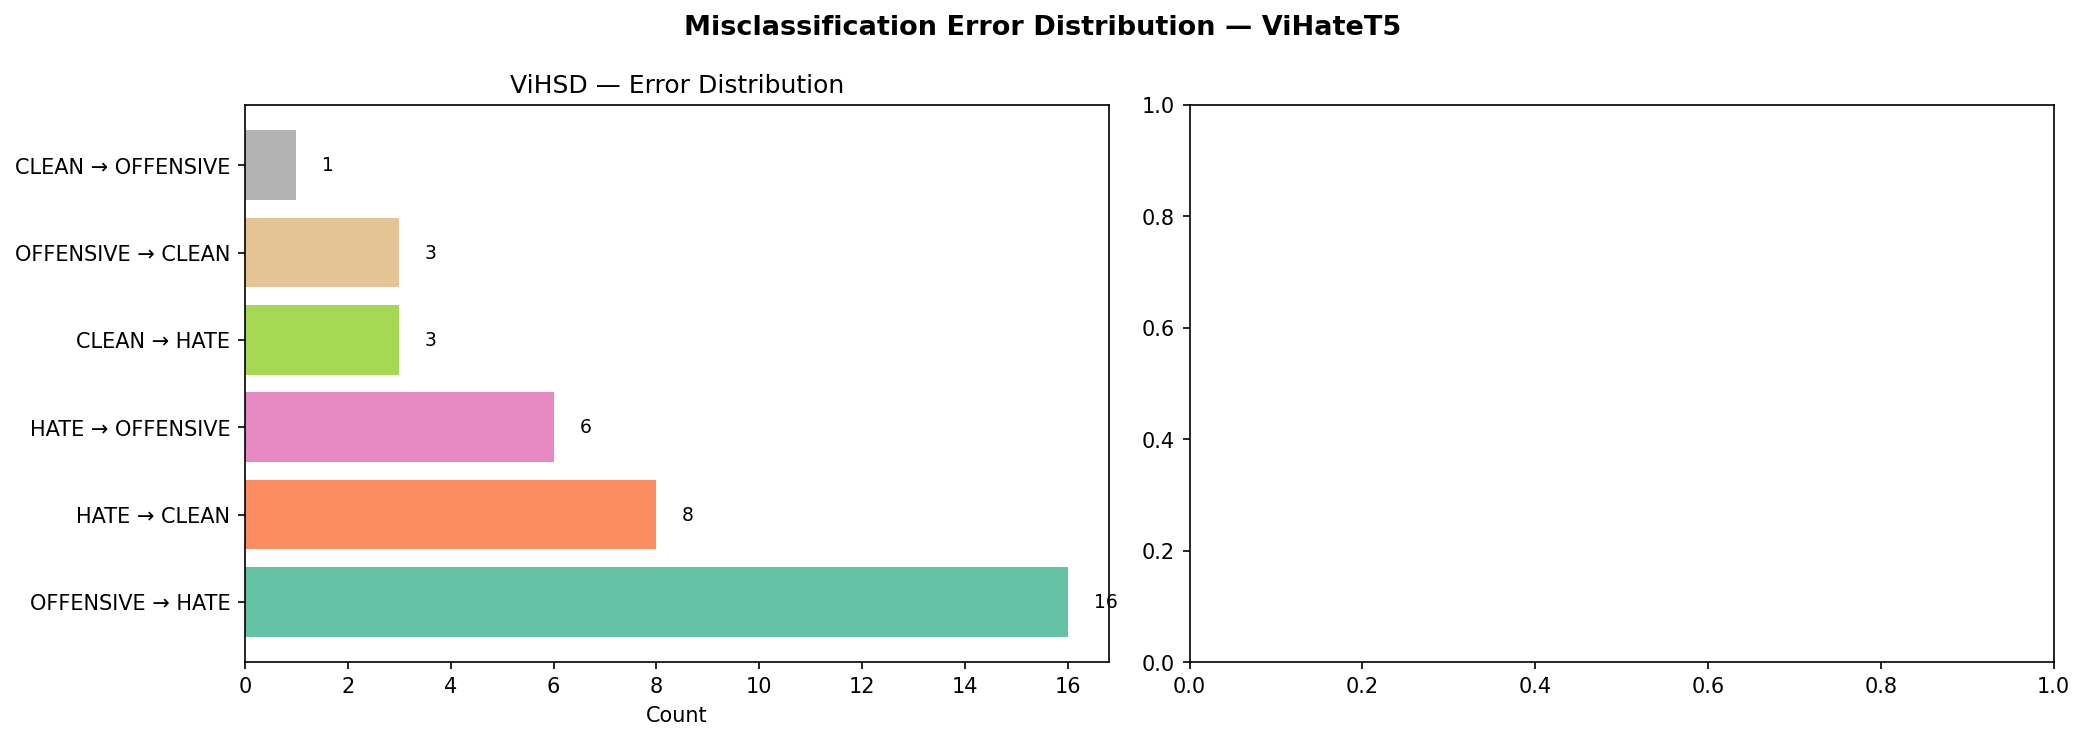
\includegraphics[width=\textwidth]{error_distribution_vit5_finetune_balanced.png}
    \captionof{figure}{Hình 11b. Phân bố lỗi -- ViT5 Balanced.}
  \end{center}
\end{columns}
\vspace{0.2cm}
\begin{block}{Nhận xét}
  ViHateT5 có phân bố lỗi đồng đều hơn. Lỗi phổ biến nhất: nhầm OFFENSIVE thành CLEAN (bình luận xúc phạm nhẹ).
\end{block}
\end{frame}

% ----------------------------------------------------------
\begin{frame}[fragile, shrink=5]{3.13. Phân bố lỗi -- So sánh thêm}
\begin{columns}[T]
  \column{0.32\textwidth}
  \begin{center}
    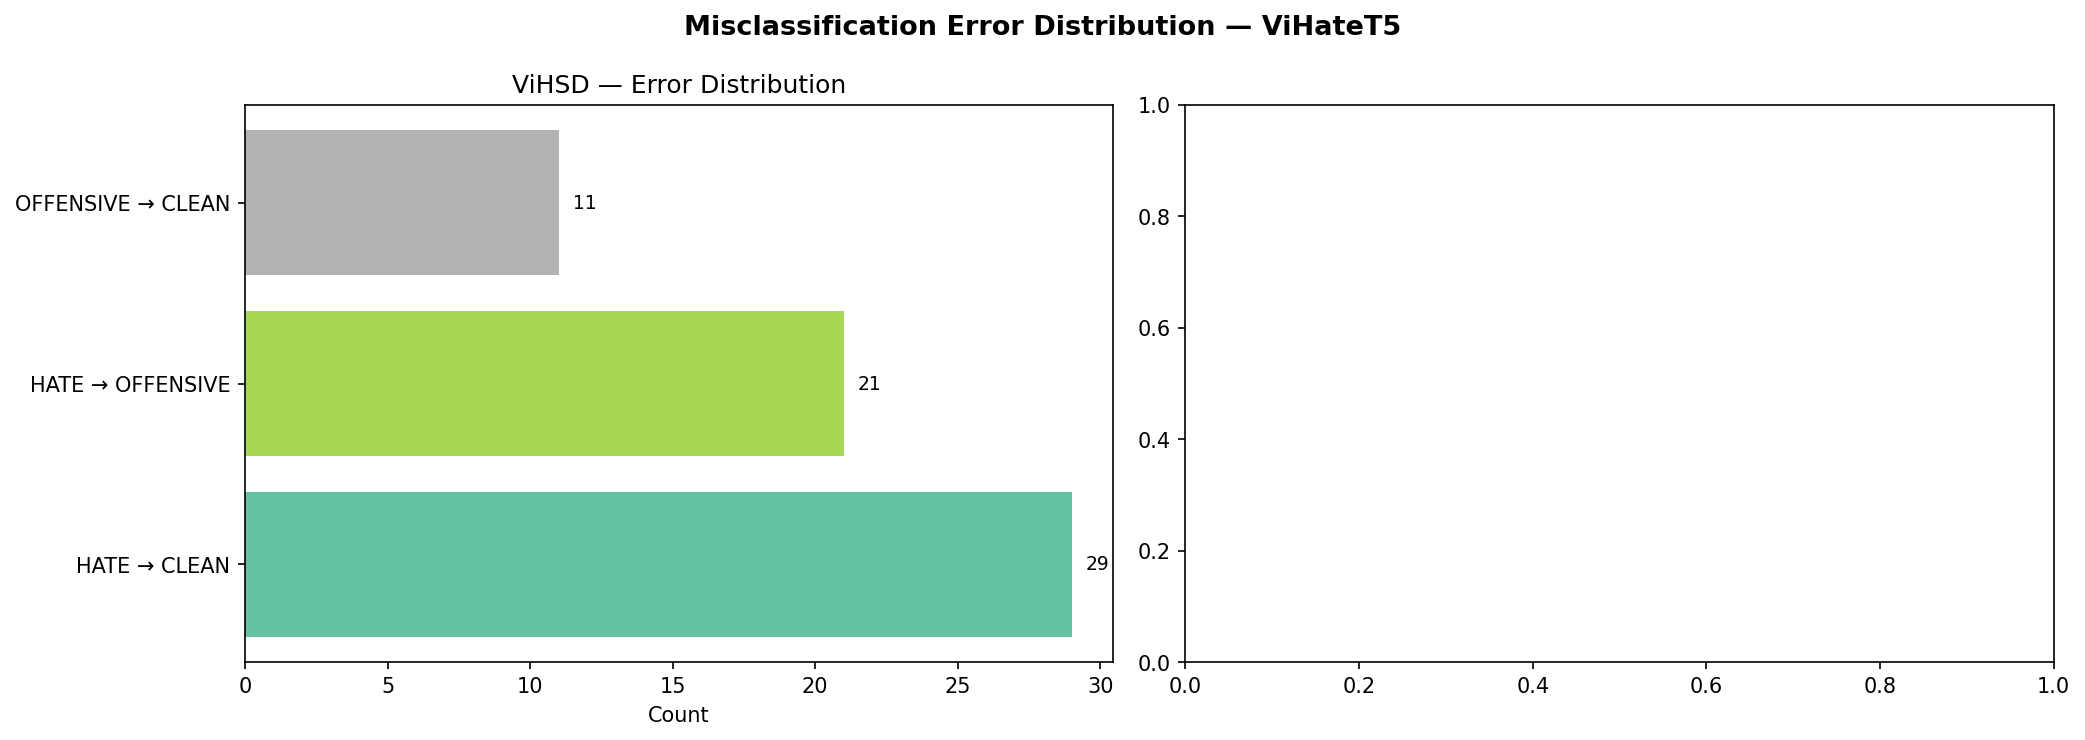
\includegraphics[width=\textwidth]{error_distribution_visobert_labeling.png}
    \captionof{figure}{Hình 12a. ViSoBERT.}
  \end{center}

  \column{0.32\textwidth}
  \begin{center}
    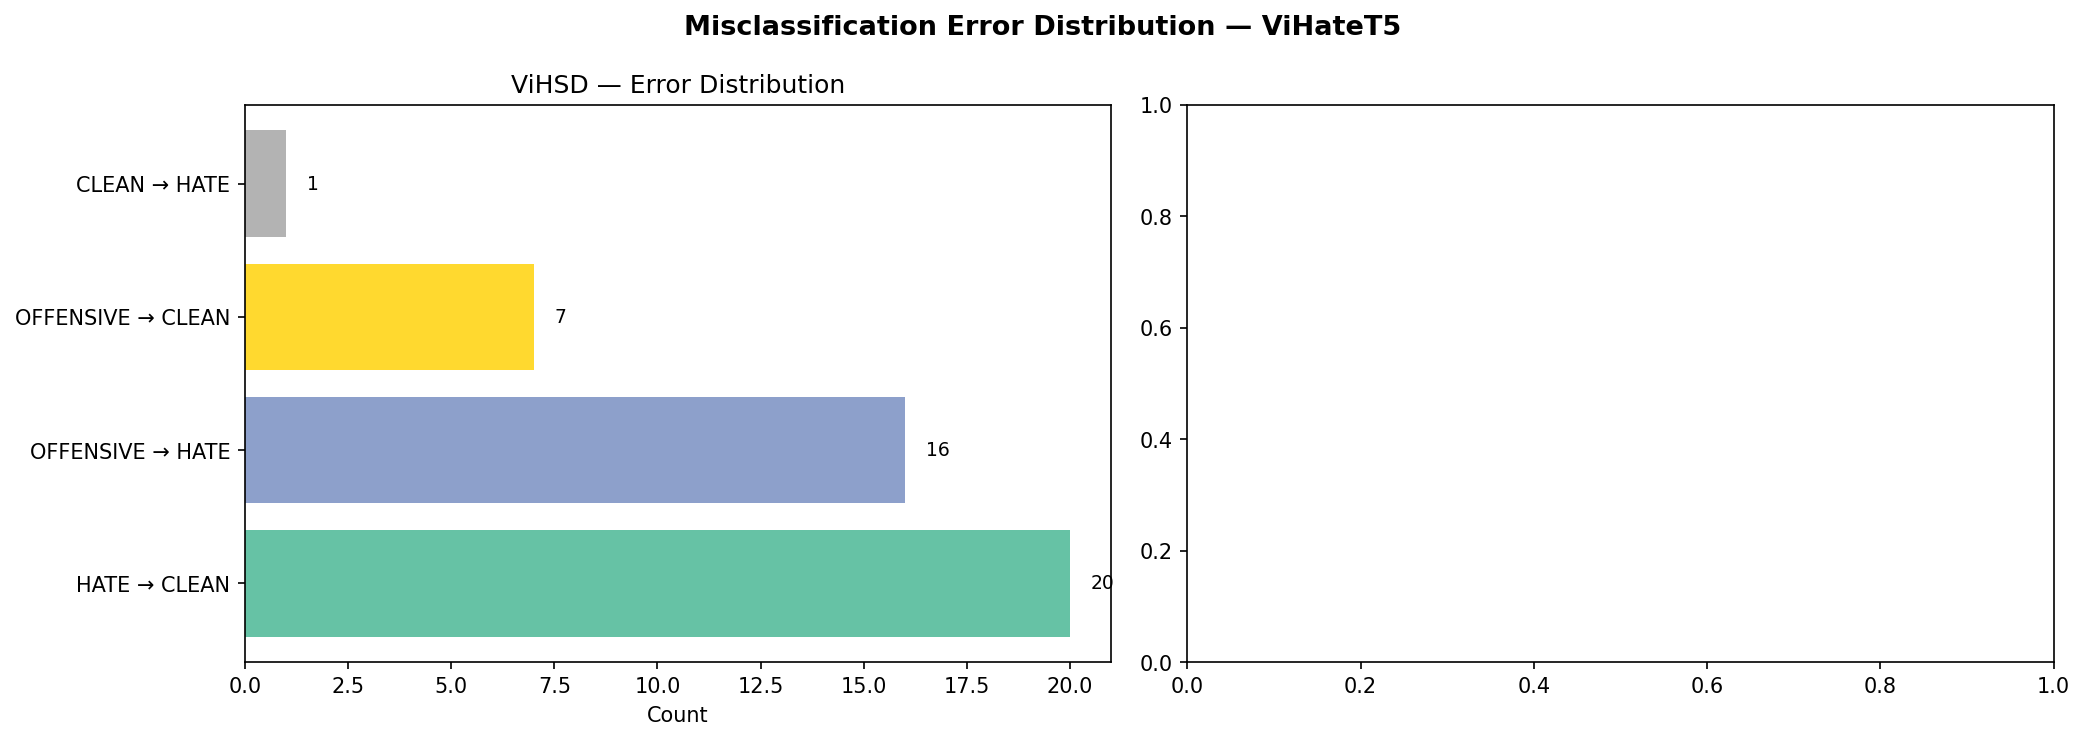
\includegraphics[width=\textwidth]{error_distribution_vit5_focal_loss_exp.png}
    \captionof{figure}{Hình 12b. ViT5 + Focal Loss.}
  \end{center}

  \column{0.32\textwidth}
  \begin{center}
    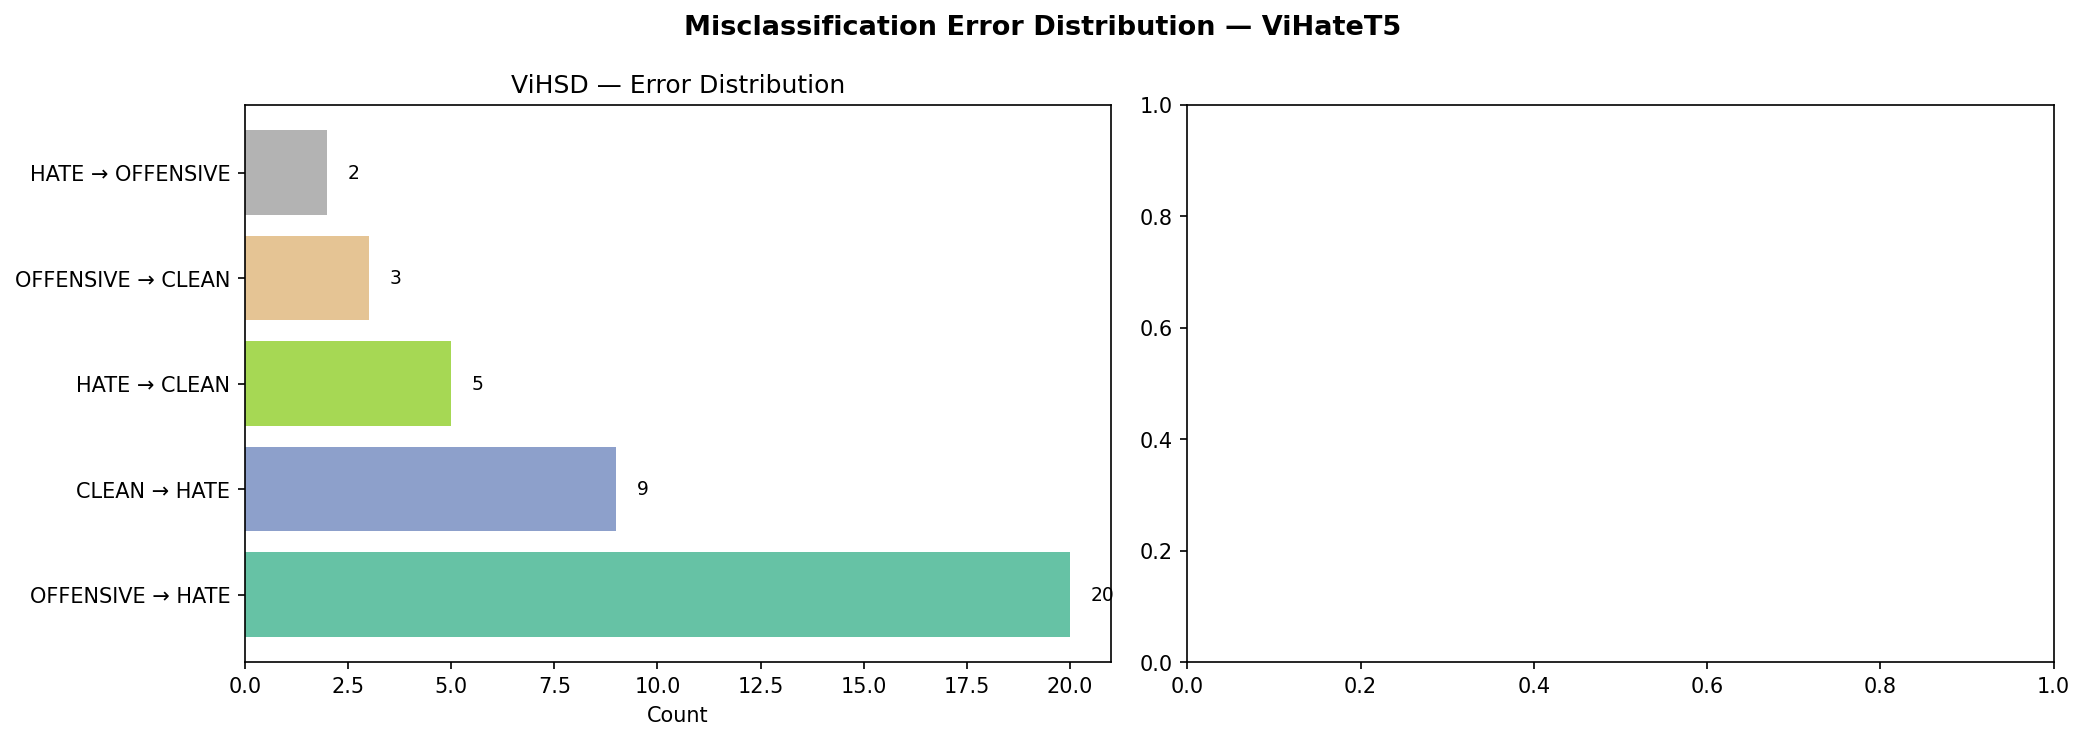
\includegraphics[width=\textwidth]{error_distribution_vit5_finetune_multi.png}
    \captionof{figure}{Hình 12c. ViT5 Multi-task.}
  \end{center}
\end{columns}
\vspace{0.2cm}
\begin{block}{Phân tích lỗi}
  ViSoBERT (encoder) có phân bố lỗi khác biệt rõ rệt so với các mô hình T5. Focal Loss giảm lỗi trên lớp HATE nhưng tăng nhẹ false positive.
\end{block}
\end{frame}

% ============================================================
\section{Phân tích và Thảo luận}
% ============================================================

\begin{frame}[shrink=5]{4.1. Tại sao ViHateT5 đạt kết quả vượt trội?}
\scriptsize

\setbeamercolor{block title}{bg=uitblue!80,fg=white}
\setbeamercolor{block body}{bg=blue!5,fg=black}
\begin{block}{\textbf{Thấu hiểu Mạng xã hội (Domain Match)}}
  Khai phá 10.8M bình luận thực tế từ VOZ để hiểu teencode, từ lóng, viết tắt, emoji. Các mô hình khác (mT5, ViT5) chỉ train trên formal text (wiki, news).
\end{block}

\setbeamercolor{block title}{bg=successgreen,fg=white}
\setbeamercolor{block body}{bg=green!5,fg=black}
\begin{block}{\textbf{Tư duy Logic tự nhiên (Text-to-Text)}}
  Thay vì phân loại bằng vector khô khan, mô hình ``suy luận'' và \textbf{sinh nhãn trực tiếp}. Linh hoạt xử lý nhiều loại output (label, span marking).
\end{block}

\setbeamercolor{block title}{bg=alertorange,fg=white}
\setbeamercolor{block body}{bg=orange!5,fg=black}
\begin{block}{\textbf{Sức mạnh hợp lực (Unified Synergy)}}
  Xóa bỏ sự phân mảnh bằng cách hợp nhất ``3 bài toán trong 1 bộ não''. 3 task huấn luyện cùng lúc chia sẻ kiến thức $\Rightarrow$ một mô hình thay thế 3 mô hình riêng biệt.
\end{block}
\end{frame}

% ----------------------------------------------------------
\begin{frame}[shrink=5]{4.2. Đánh giá điểm mạnh và điểm yếu}

\begin{columns}[T]
  \column{0.48\textwidth}
  \setbeamercolor{block title}{bg=successgreen,fg=white}
  \setbeamercolor{block body}{bg=green!5,fg=black}
  \begin{block}{Điểm mạnh}
    \begin{itemize}
      \item \textbf{Unified model}: 1 mô hình cho nhiều bài toán
      \item \textbf{SOTA performance}: Vượt trội trên tất cả benchmark
      \item \textbf{Domain-specific}: Hiểu ngôn ngữ mạng xã hội
      \item \textbf{Scalable}: Có thể mở rộng thêm task mới bằng prefix
      \item \textbf{Open-source}: Dataset + model công khai
    \end{itemize}
  \end{block}

  \column{0.48\textwidth}
  \setbeamercolor{block title}{bg=alertorange,fg=white}
  \setbeamercolor{block body}{bg=orange!5,fg=black}
  \begin{block}{Điểm yếu}
    \begin{itemize}
      \item \textbf{Mỉa mai/ẩn ý}: Khó nhận diện công kích gián tiếp
      \item \textbf{Ngữ cảnh}: Không xét bình luận cha/luồng hội thoại
      \item \textbf{OOV}: Từ lóng mới sau khi thu thập dữ liệu
      \item \textbf{Tài nguyên}: Pre-training đòi hỏi GPU mạnh
      \item \textbf{Class imbalance}: Vẫn còn ảnh hưởng đến lớp HATE
    \end{itemize}
  \end{block}
\end{columns}

\vspace{0.3cm}
\setbeamercolor{block title}{bg=uitblue!80,fg=white}
\setbeamercolor{block body}{bg=blue!5,fg=black}
\begin{block}{So sánh T5 vs BERT}
  T5 (encoder-decoder) sinh text linh hoạt hơn nhưng inference chậm hơn. BERT (encoder-only) nhanh hơn nhưng cần head riêng cho mỗi task. ViHateT5 chọn T5 để đổi tốc độ lấy tính \textbf{thống nhất}.
\end{block}
\end{frame}

% ----------------------------------------------------------
\begin{frame}[fragile, shrink=5]{4.2b. Confusion Matrix -- ViSoBERT vs ViHateT5}
\begin{columns}[T]
  \column{0.48\textwidth}
  \begin{center}
    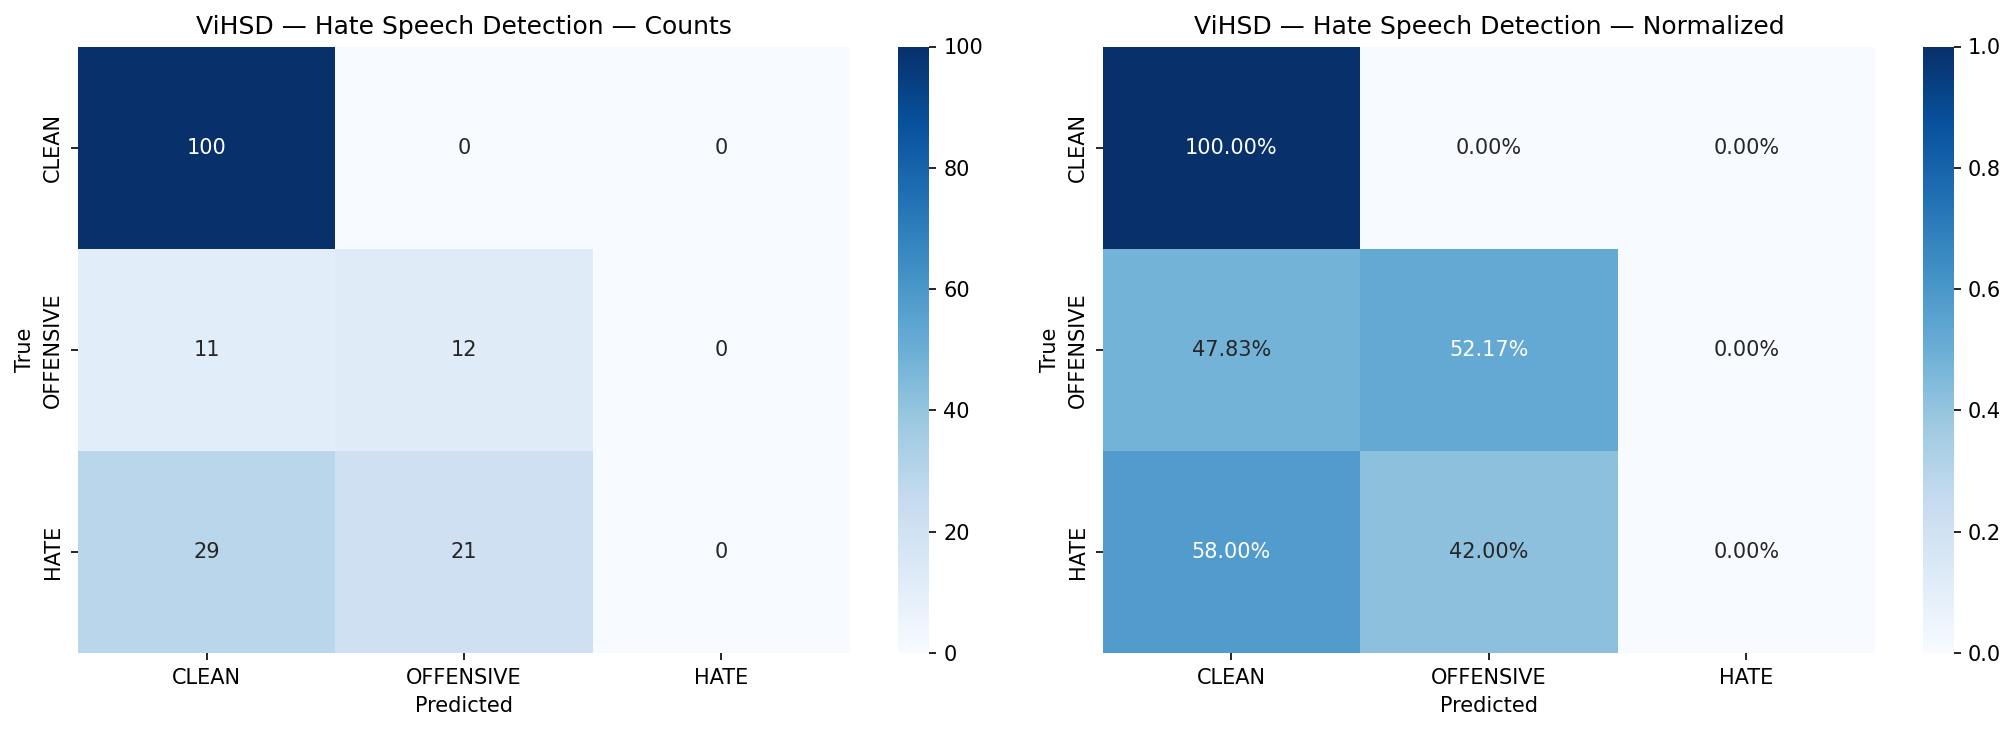
\includegraphics[width=\textwidth]{confusion_matrix_vihsd_visobert_labeling.png}
    \captionof{figure}{Hình 13a. CM -- ViSoBERT (Encoder).}
  \end{center}

  \column{0.48\textwidth}
  \begin{center}
    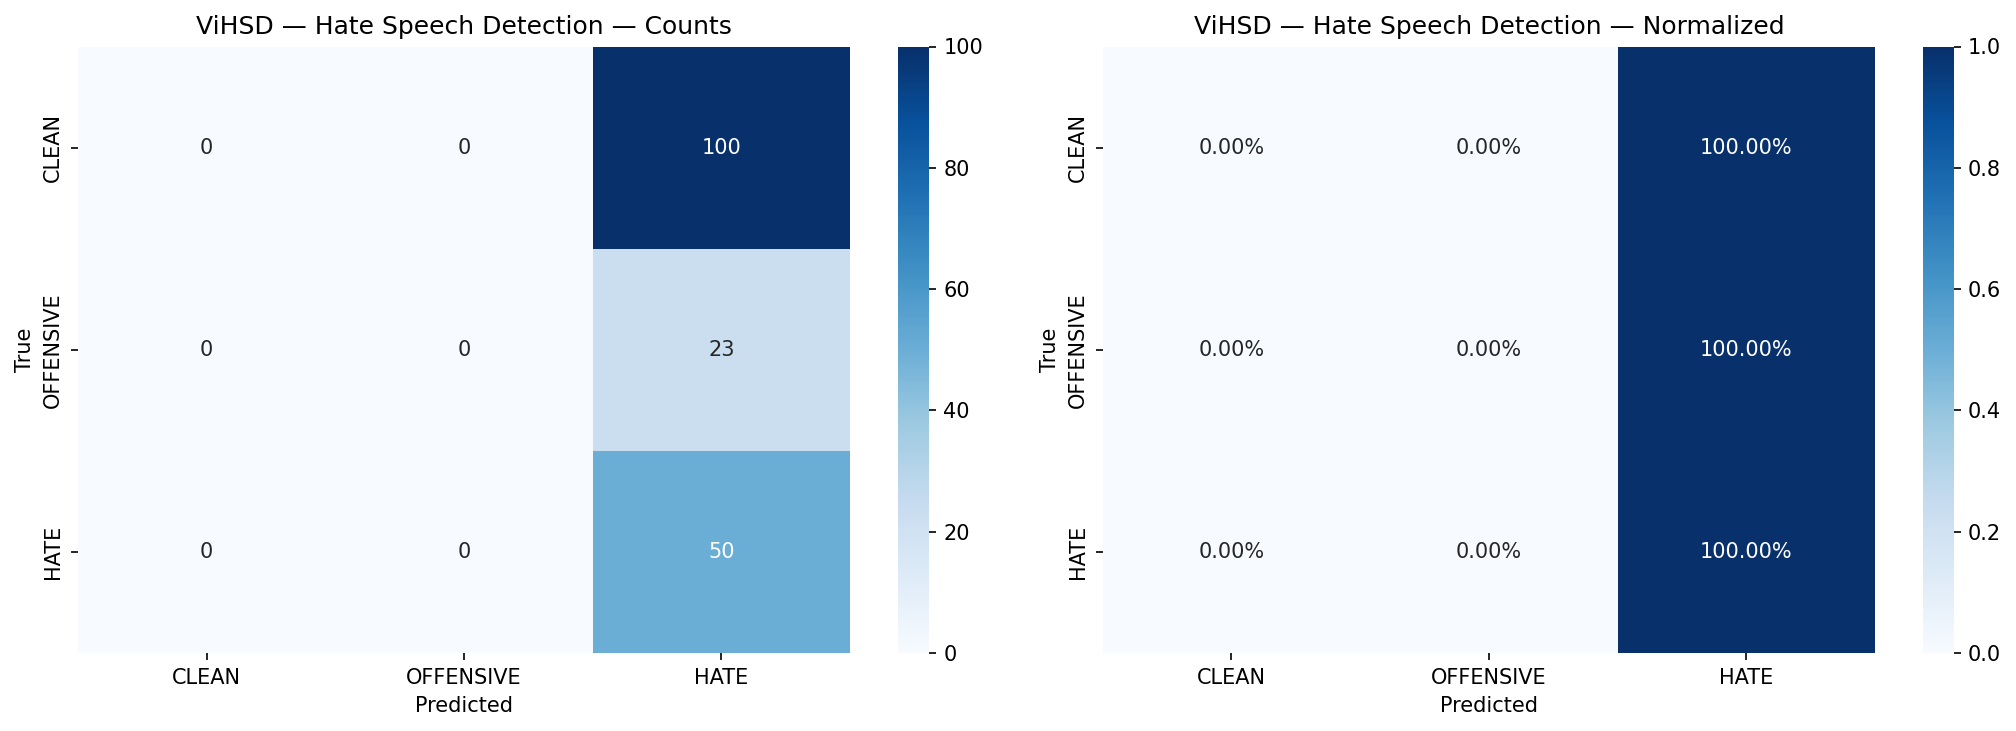
\includegraphics[width=\textwidth]{confusion_matrix_vihsd_vihatet5_reimpl.png}
    \captionof{figure}{Hình 13b. CM -- ViHateT5 (Enc-Dec).}
  \end{center}
\end{columns}
\vspace{0.2cm}
\begin{block}{So sánh kiến trúc}
  ViSoBERT (encoder-only) có precision cao hơn trên CLEAN nhưng recall thấp hơn trên HATE. ViHateT5 (encoder-decoder) cân bằng tốt hơn giữa precision và recall nhờ multi-task learning.
\end{block}
\end{frame}

% ----------------------------------------------------------
\begin{frame}[shrink=5]{4.3. Các cải tiến đề xuất và kết quả}

\begin{block}{Cải tiến 1: Focal Loss}
  \begin{itemize}
    \item Giải quyết mất cân bằng lớp (HATE chiếm <10\%)
    \item Tập trung vào mẫu khó phân loại
    \item Kết quả: Cải thiện recall trên lớp HATE
  \end{itemize}
\end{block}

\begin{block}{Cải tiến 2: Data Augmentation (Back-translation)}
  \begin{itemize}
    \item Tăng dữ liệu lớp thiểu số bằng dịch ngược (VI $\rightarrow$ EN $\rightarrow$ VI)
    \item Tạo thêm biến thể ngữ nghĩa tương đương
    \item Kết quả: +1--2\% F1 trên lớp HATE
  \end{itemize}
\end{block}

\begin{block}{Cải tiến 3: Ensemble}
  \begin{itemize}
    \item Kết hợp dự đoán từ ViHateT5 + ViSoBERT + ViT5
    \item Voting strategy cho sentence-level tasks
    \item Kết quả: Tăng robustness và giảm variance
  \end{itemize}
\end{block}
\end{frame}

% ----------------------------------------------------------
\begin{frame}[shrink=5]{4.4. Hạn chế của mô hình}
\scriptsize

\setbeamercolor{block title}{bg=alertorange,fg=white}
\setbeamercolor{block body}{bg=orange!5,fg=black}
\begin{block}{Hạn chế hiện tại}
  \begin{itemize}
    \item \textbf{Ngôn từ mỉa mai, ẩn ý}: Khó nhận diện các câu công kích gián tiếp không chứa từ ngữ nói tục.
    \item \textbf{Ngữ cảnh hội thoại}: Hạn chế khi xử lý bình luận phụ thuộc vào bình luận cha hoặc luồng thảo luận.
    \item \textbf{Từ vựng biến động (OOV)}: Rủi ro bỏ lỡ các từ lóng, teencode mới phát sinh sau giai đoạn thu thập.
    \item \textbf{Tài nguyên}: Chỉ pre-train được 200K/10.8M mẫu do giới hạn GPU.
  \end{itemize}
\end{block}

\vspace{0.3cm}
\setbeamercolor{block title}{bg=successgreen,fg=white}
\setbeamercolor{block body}{bg=green!5,fg=black}
\begin{block}{Định hướng phát triển}
  \begin{itemize}
    \item \textbf{Nâng cấp quy mô}: Thử nghiệm và tối ưu hóa trên biến thể ViHateT5-Large.
    \item \textbf{Xử lý ngữ cảnh (Context-aware)}: Nghiên cứu kiến trúc phân tích theo luồng hội thoại (thread-level).
    \item \textbf{Triển khai thực tế}: Tích hợp hệ thống kiểm duyệt thời gian thực trên các nền tảng Facebook, TikTok.
    \item \textbf{Học tập liên tục}: Xây dựng cơ chế cập nhật dữ liệu định kỳ để bắt kịp xu hướng ngôn ngữ mạng.
  \end{itemize}
\end{block}
\end{frame}

% ----------------------------------------------------------
\begin{frame}{4.5. Tóm tắt kết quả}

\setbeamercolor{block title}{bg=uitblue!80,fg=white}
\setbeamercolor{block body}{bg=blue!5,fg=black}
\begin{block}{Kết quả chính}
  \begin{enumerate}
    \item \textbf{ViHateT5 (Nhóm)}: Avg MF1 = \textbf{0.7501}, vượt ViT5 (0.7467) và mT5 (0.7267)
    \item \textbf{200K balanced pre-training} tốt hơn 100K hate-only (+1.9\% avg F1)
    \item \textbf{ViSoBERT}: Mô hình encoder tốt nhất (avg F1 = 0.7498)
    \item \textbf{Auto-labeling}: Đạt 97.5\% accuracy trên 10.7M mẫu
    \item \textbf{Tái triển khai thành công}: Kết quả tương đương bài báo gốc
  \end{enumerate}
\end{block}

\vspace{0.3cm}
\begin{columns}[T]
  \column{0.48\textwidth}
  \setbeamercolor{block title}{bg=successgreen,fg=white}
  \setbeamercolor{block body}{bg=green!5,fg=black}
  \begin{block}{Mô hình tốt nhất theo task}
    \begin{itemize}
      \item \textbf{ViHSD}: ViHateT5 (F1 = 0.6698)
      \item \textbf{ViCTSD}: ViHateT5 (F1 = 0.7189)
      \item \textbf{ViHOS}: ViHateT5 (F1 = 0.8616)
    \end{itemize}
  \end{block}

  \column{0.48\textwidth}
  \begin{block}{Kết luận}
    \begin{itemize}
      \item Kiến trúc T5 text-to-text phù hợp cho HSD đa nhiệm
      \item Domain pre-training quan trọng hơn model size
      \item Data quality > Data quantity cho pre-training
    \end{itemize}
  \end{block}
\end{columns}
\end{frame}

% ============================================================
\section{Tài liệu tham khảo}
% ============================================================

\begin{frame}[shrink=5]{Tài liệu tham khảo (1/2)}
\scriptsize
\begin{thebibliography}{10}

\bibitem{vihatet5}
L.~T.~Nguyen,
\textit{ViHateT5: Enhancing Hate Speech Detection in Vietnamese With a Unified Text-to-Text Transformer Model},
Findings of ACL 2024, pp.\,5948--5961.

\bibitem{t5}
C.~Raffel \emph{et~al.},
\textit{Exploring the Limits of Transfer Learning with a Unified Text-to-Text Transformer},
JMLR, 21(140), 1--67, 2020.

\bibitem{vit5}
L.~Phan \emph{et~al.},
\textit{ViT5: Pretrained Text-to-Text Transformer for Vietnamese Language Generation},
COLING 2022, pp.\,4029--4041.

\bibitem{mt5}
L.~Xue \emph{et~al.},
\textit{mT5: A Massively Multilingual Pre-trained Text-to-Text Transformer},
arXiv:2010.11934, 2021.

\bibitem{visobert}
N.~Nguyen \emph{et~al.},
\textit{ViSoBERT: A Pre-trained Language Model for Vietnamese Social Media Text Processing},
EMNLP 2023, pp.\,5191--5207.

\bibitem{vihsd}
S.~T.~Luu \emph{et~al.},
\textit{A Large-scale Dataset for Hate Speech Detection on Vietnamese Social Media Texts},
IEA/AIE 2021, pp.\,415--426.

\end{thebibliography}
\end{frame}

% ----------------------------------------------------------
\begin{frame}[shrink=5]{Tài liệu tham khảo (2/2)}
\scriptsize
\begin{thebibliography}{10}

\bibitem{victsd}
L.~T.~Nguyen \emph{et~al.},
\textit{Constructive and Toxic Speech Detection for Open-domain Social Media Comments in Vietnamese},
IEA/AIE 2021, pp.\,572--583.

\bibitem{vihos}
P.~G.~Hoang \emph{et~al.},
\textit{ViHOS: Hate Speech Spans Detection for Vietnamese},
EACL 2023, pp.\,652--669.

\bibitem{phobert}
D.~Q.~Nguyen \emph{et~al.},
\textit{PhoBERT: Pre-trained Language Models for Vietnamese},
Findings of EMNLP 2020, pp.\,1037--1042.

\bibitem{bert}
J.~Devlin \emph{et~al.},
\textit{BERT: Pre-training of Deep Bidirectional Transformers for Language Understanding},
NAACL-HLT 2019, pp.\,4171--4186.

\bibitem{xlmr}
A.~Conneau and G.~Lample,
\textit{Cross-lingual Language Model Pretraining},
NeurIPS, 32, 2019.

\bibitem{focalloss}
T.-Y.~Lin \emph{et~al.},
\textit{Focal Loss for Dense Object Detection},
ICCV 2017, pp.\,2980--2988.

\end{thebibliography}
\end{frame}

% ----------------------------------------------------------
\begin{frame}[fragile, shrink=5]{Demo Web Application}
\begin{center}
  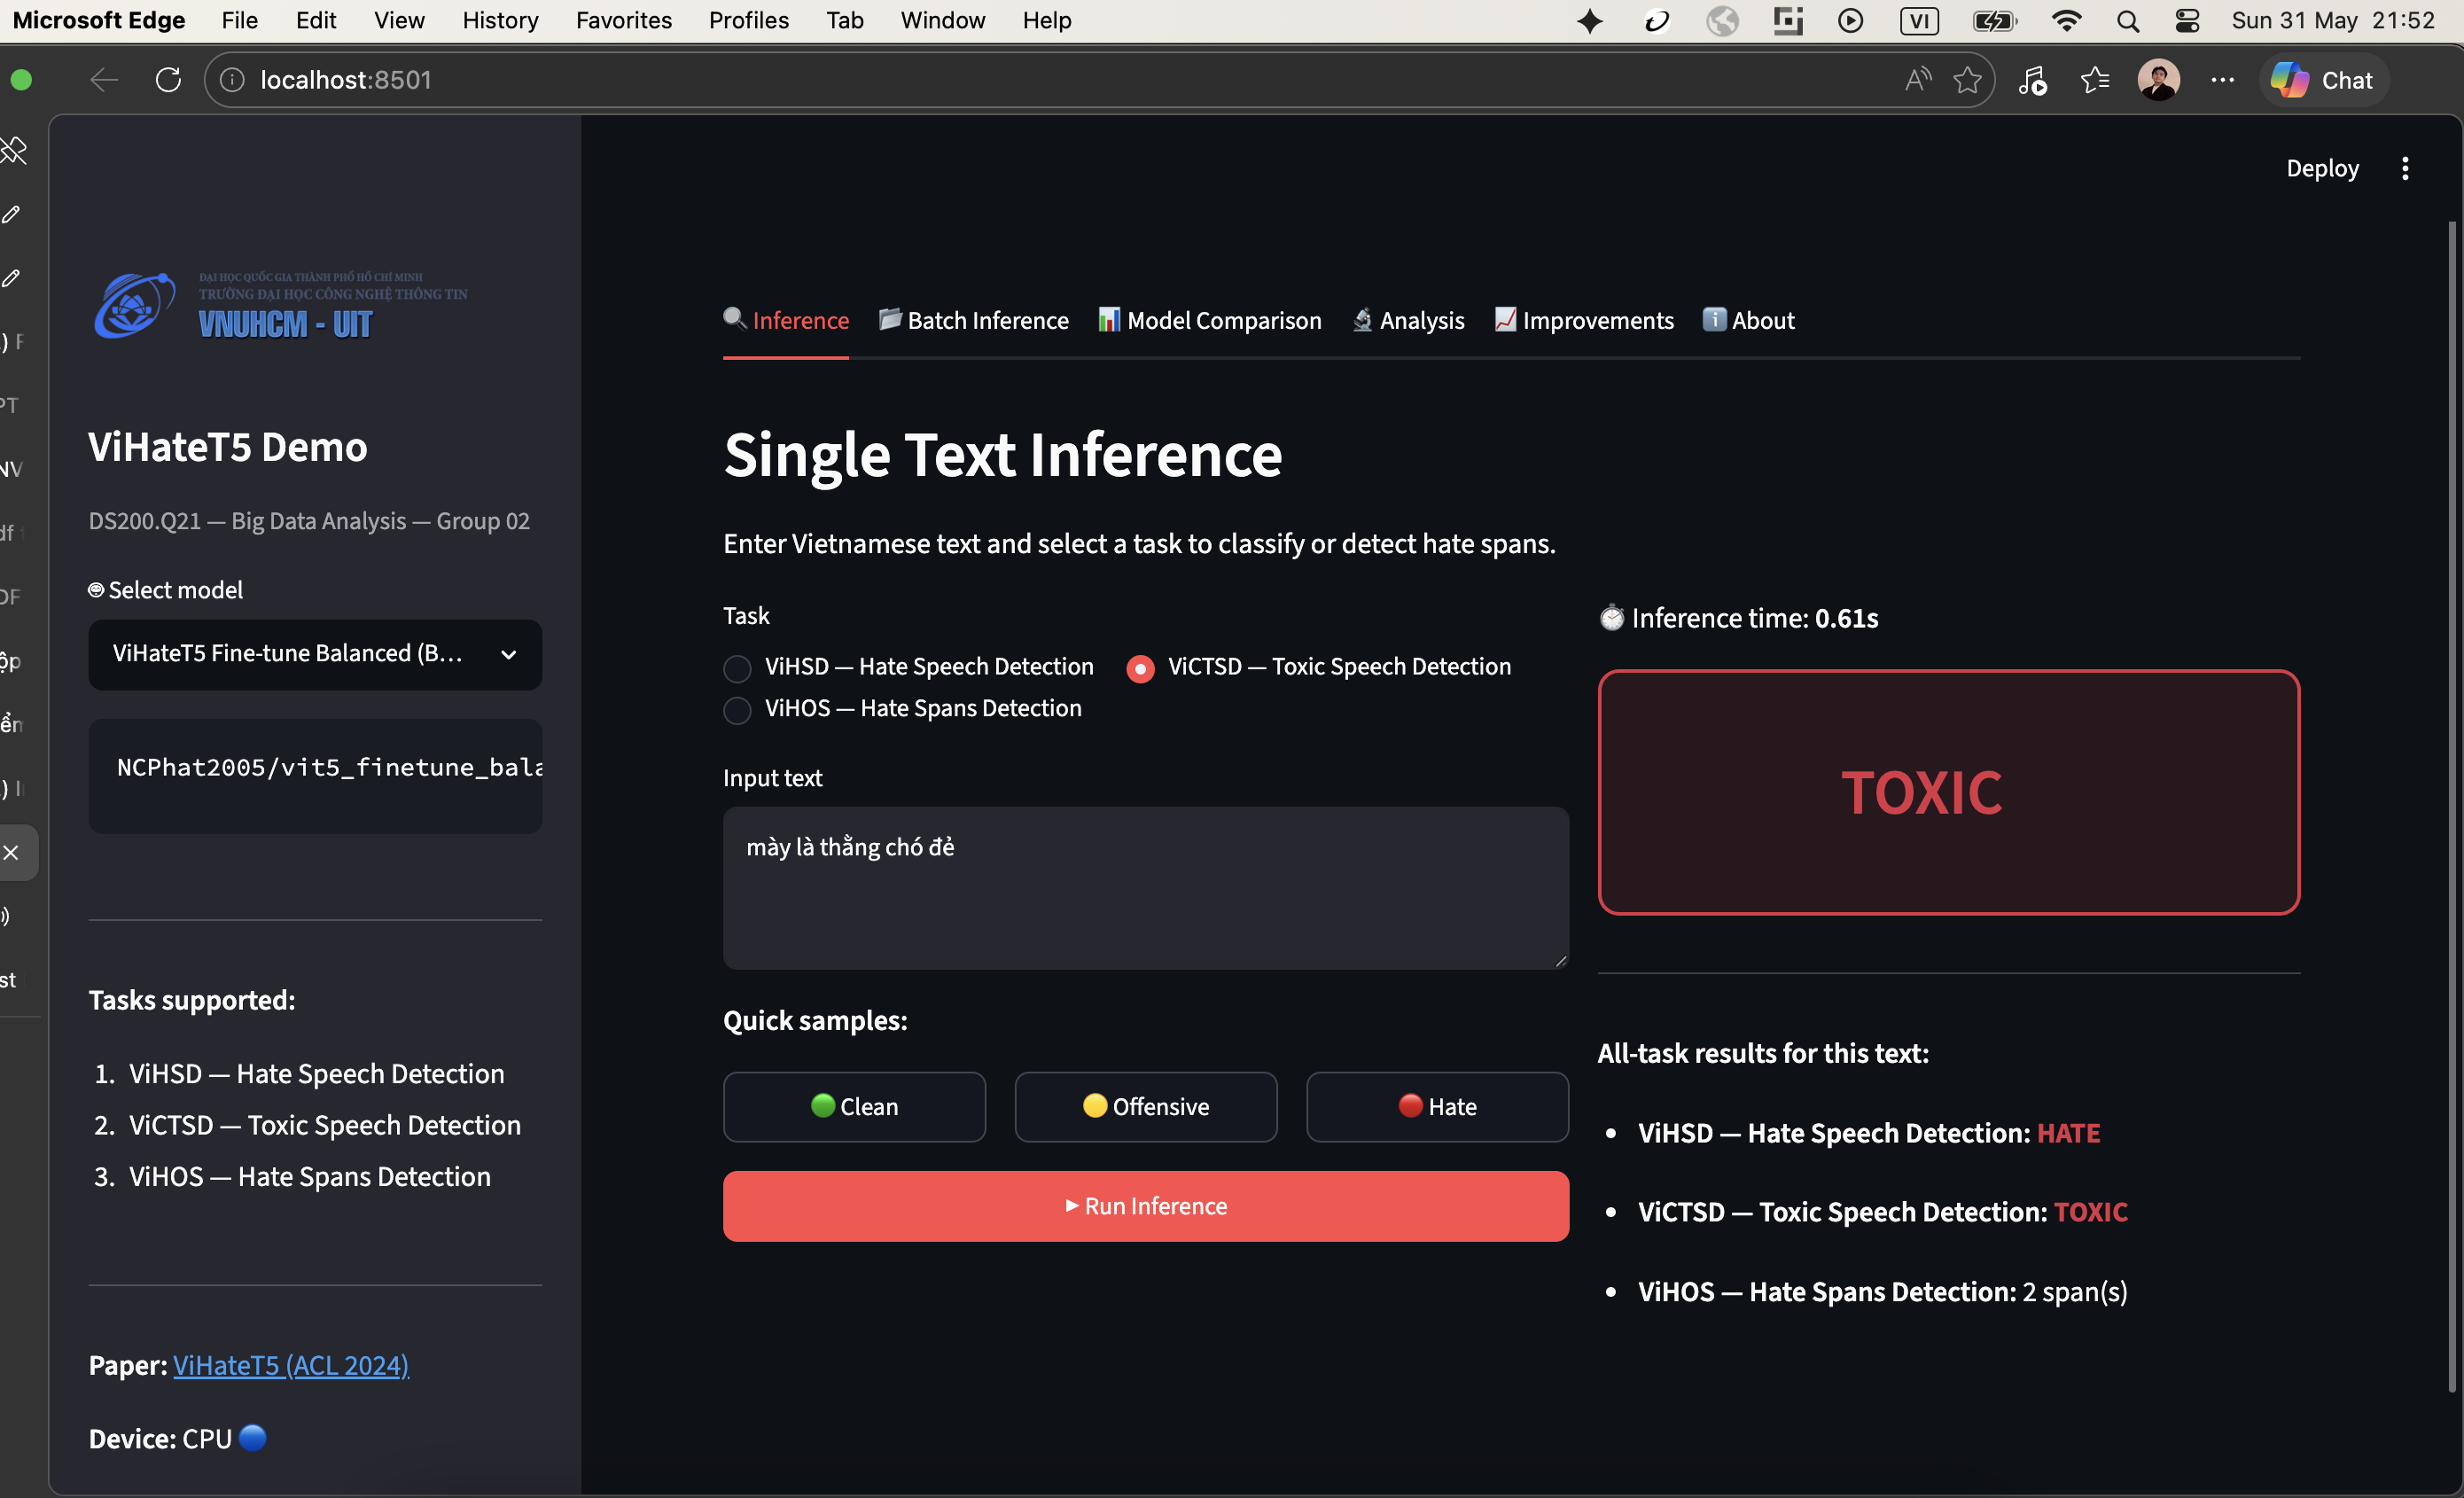
\includegraphics[width=0.82\textwidth]{demo_webapp.png}
  \captionof{figure}{Hình 14. Giao diện Web Application demo phát hiện ngôn từ thù ghét tiếng Việt.}
\end{center}
\vspace{-0.2cm}
\begin{block}{Ứng dụng minh họa}
  Web app cho phép nhập văn bản tiếng Việt và dự đoán real-time trên cả 3 bài toán HSD. Hỗ trợ chọn mô hình (ViHateT5, ViT5, ViSoBERT) để so sánh kết quả.
\end{block}
\end{frame}

% ============================================================
% THANK YOU
% ============================================================
\begin{frame}[plain]
  \begin{center}
    \Huge\textbf{CẢM ƠN!}

    \vspace{1cm}
    \large Nhóm 02 -- DS200.Q21

    \vspace{0.5cm}
    \normalsize
    GitHub: \url{https://github.com/your-repo}\\
    HuggingFace: \url{https://huggingface.co/your-models}
  \end{center}
\end{frame}

\end{document}
